\documentclass[journal]{IEEEtran}
\usepackage[T1]{fontenc}
\usepackage[utf8]{inputenc}
\usepackage{graphicx}
\usepackage{booktabs}
\usepackage{amsmath}
\usepackage{array}
\usepackage{longtable}
\usepackage{tabularx}
\usepackage{multirow}
\usepackage{enumitem}
\usepackage[hidelinks]{hyperref}
\usepackage{url}
\graphicspath{{../figures/main6/}}
\newcolumntype{Y}{>{\raggedright\arraybackslash}X}
\newcolumntype{L}[1]{>{\raggedright\arraybackslash}p{#1}}
\begin{document}
\title{Cross-View Identity in Image-Based Fruit Counting: A Systematic Review and Design Space for Class-Wise Inventories}
\author{Muhammad~Zainal~Muttaqin and Fatma~Indriani%
\thanks{Department of Computer Science, Universitas Lambung Mangkurat, Banjarbaru, Indonesia.}}
\maketitle
\begin{abstract}
A fruit inventory built from photographs must count each physical fruit once, although a camera moving along a row or around a tree sees most fruit several times. This systematic review asks which mechanisms decide that observations in different images belong to the same fruit, what evidence supports each, and how class labels such as maturity are attached to the unique fruit. Scopus was searched on 28 September 2026 with thirteen reproducible query runs covering 2012--2026. Of 5{,}889 unique records, 971 studies were mapped, including 187 that combine several observations of the same fruit and 170 on oil-palm fresh fruit bunches. The 187 multi-observation studies were coded into six mechanisms: no association, statistical correction, appearance matching, temporal tracking, geometric or 3D association, and learned association. Tracking appears in 62\% of the 182 method studies and geometric association in 37\%; learned association appears in three. Only 19 report counts per class, and 18 of the 140 with an abstract report an identity metric. Where designs were compared on the same trees, one image of one or both sides counted 27--58\% of the fruit, and tracking or 3D association raised this while adding duplicates of their own; on look-alike fruit, trackers using appearance features did not outperform motion-only trackers. Of the 170 oil-palm studies, 76 classify the ripeness of single-bunch images, nine count bunches, and one dataset links bunches across views of a palm. The review states the acquisition assumptions of each mechanism and the measurements needed to test a duplicate-aware, class-wise inventory.
\end{abstract}
\begin{IEEEkeywords}
fruit counting, multi-view perception, multi-object tracking, data association, structure from motion, yield estimation, oil palm, systematic review
\end{IEEEkeywords}
\section{Introduction}\label{sec:intro}

A grower who needs the number of ripe fruit on a block wants one record for each physical fruit, with its class. A camera does not supply that record. It supplies images, and in most field protocols the same fruit appears in several of them: in consecutive video frames, in photographs taken from both sides of a row, or in images taken while walking around a single tree. Detection finds fruit in each image. It does not say whether a fruit found in one image is the fruit found in another. The step that makes that decision determines whether a sum of detections is an inventory or an overcount.

The size of the problem is known from studies that measured it directly. In a mango orchard, one image of each side of 16 trees counted 54\% of the fruit that were hand-counted, and one image of one side counted 27\%; tracking every fruit through a multi-view sequence and triangulating it counted 101.4\% \citep{stein2016image}. On 21 mango trees, video tracking recorded 62\% of the harvest count and two images per tree recorded 40\% \citep{wang2019mango}. On a 192-fruit video, the same tracker produced 9.9\% double counts and 7.3\% missed fruit, which netted to a 2.6\% overcount \citep{wang2019mango}. The last figure shows why a total count can look correct when the underlying identity decisions are not: a duplicate and a miss cancel.

In oil palm the problem takes a specific form. Plantations estimate output with a bunch census in which staff count and classify bunches on each palm by the number of months until harvest. The SawitMVC dataset photographed 953 palms from four or eight sides and annotated 9{,}823 unique bunches in four census classes, with links that record which boxes in different images show the same bunch \citep{indriani2026sawitmvc}. A census built from such photographs needs both the identity decision and a class label for each unique bunch.

From the perspective of counting unique fruit, earlier reviews leave three things open. First, they organize the literature by sensor \citep{gongal2015sensors,fu2020application}, by detector family \citep{koirala2019deepb,huang2023survey}, by yield-estimation route \citep{anderson2021technologies,he2022fruit}, or, for oil palm, by ripeness-sensing method \citep{lai2023oil,goh2025fresh}; none takes the identity of a fruit across observations as the organizing variable, although several discuss occlusion and extrapolation from partial counts. Second, reviews of tracking, re-identification, and 3D reconstruction outside agriculture provide the mechanisms but not the agricultural evidence. Third, five of the eleven closest reviews do not state how their studies were found, and two more describe themselves as systematic without reporting databases or search strings (Table~\ref{tab:position}). As a result, a reader cannot tell which association mechanism fits a given acquisition protocol, or what evidence supports it.

To address these issues, this article presents a systematic mapping review of image-based fruit counting published between 2012 and 2026. Reporting follows PRISMA~2020 where its items apply to a mapping review. Scopus was the single database, searched on 28 September 2026, and \nIncluded studies are included, of which \nMulti combine several observations of the same fruit.

This review makes three contributions. First, it provides a systematic map of the \nIncluded studies, with the search strings reported in full and the screening decisions, the codes, and the log of changes made during verification provided as supplementary material. Second, it defines a design space that separates acquisition, observation, association, attribute assignment, and inventory, and classifies association into six mechanisms (no association, statistical correction, appearance matching, temporal tracking, geometric or 3D association, and learned association), each tied to the conditions it assumes. Third, it synthesizes the \nMulti multi-observation studies by mechanism, with the comparisons that were made on the same data reported in two tables, followed by the evidence on class attributes, depth, and oil palm.

Accordingly, the review addresses four questions:
\begin{enumerate}[label=(\arabic*),leftmargin=*]
\item Which mechanisms have been used to decide that observations in different images belong to the same fruit, and what acquisition conditions does each assume?
\item What evidence shows how well each mechanism controls duplicates and misses, and how was that evidence measured?
\item How are class attributes, mainly maturity, attached to a unique fruit rather than to each detection?
\item What does the oil-palm imaging literature cover, and what is missing for a bunch-level, class-wise census from images?
\end{enumerate}

The remainder of this article is organized as follows. Section~\ref{sec:method} describes the search, screening, and coding. Section~\ref{sec:framework} sets out the design space and reports how the multi-observation studies are distributed over it. Sections~\ref{sec:acq} to~\ref{sec:class} follow its stages: acquisition (Section~\ref{sec:acq}), association, mechanism by mechanism (Section~\ref{sec:mech}), and class attributes on unique fruit (Section~\ref{sec:class}). Section~\ref{sec:depth} examines depth and other sensing modalities, and Section~\ref{sec:palm} the oil-palm case. Section~\ref{sec:position} places the review against earlier reviews, Section~\ref{sec:agenda} draws the gaps and a measurement agenda, Section~\ref{sec:limits} states the limitations, and Section~\ref{sec:conclusion} concludes.

\section{Review method}\label{sec:method}

The review is a systematic mapping review with a configurative synthesis \citep{petersen2015mapping,grant2009typology}. It maps a broad body of work and builds a classification from it; it does not pool effect sizes, because the included studies use different crops, references, and metrics. Reporting follows the Preferred Reporting Items for Systematic Reviews and Meta-Analyses (PRISMA~2020) where the items apply to a mapping review \citep{page2021prisma,page2021elaboration}, together with general guidance on reporting literature reviews written for management and transport research \citep{kraus2022,vanwee2016howto}. The workflow comprised (i) defining the four questions and the scope, (ii) specifying inclusion and exclusion criteria, (iii) searching Scopus, (iv) screening records in two stages, (v) coding the included studies, and (vi) appraising and synthesizing the evidence.

\subsection{Data source}
Scopus was used as the single bibliographic database because it indexes the journals and proceedings in which agricultural engineering and computer vision work is published, including those of Elsevier, IEEE, Springer, MDPI, and Frontiers. The search was run on 28 September 2026 (UTC).

\subsection{Search strategy}
The search comprised 13 search strings in nine query sets (Table~\ref{tab:queries}). Five sets target agricultural fruit perception: multi-observation counting, counting in titles, oil-palm imaging, class attributes with counting, and depth or 3D sensing. Two sets retrieve reviews: methods reviews on multi-object tracking (MOT), re-identification (re-ID), multi-view detection, and reconstruction, and agricultural reviews on fruit detection and yield. Two sets retrieve methods papers from outside agriculture; their results were sorted by citation count and only the 25 most cited records of each search were retained, because their role is to identify the transferable mechanisms, not to map those fields. All searches were limited to 2012--2026 and to subject areas that publish engineering or agricultural work. The complete search strings are given in Appendix~\ref{app:queries} under the keys shown in Table~\ref{tab:queries}.

\begin{table}[!t]
\centering
\caption{Scopus query sets and number of records returned and retained.}\label{tab:queries}
\footnotesize
\begin{tabularx}{\linewidth}{@{}L{2.5cm}Yrr@{}}
\toprule
Query set (key) & Search terms & Returned & Retained\\
\midrule
Multi-observation counting (Q1) & Fruit or crop terms AND counting or yield AND multi-view, video, tracking, SfM, SLAM, duplicates & 871 & 871\\
Counting in titles (Q2) & Fruit AND counting or load in the title & 757 & 757\\
Oil-palm imaging (Q3) & Oil palm or FFB AND imaging, learning, ripeness, or counting & 1{,}079 & 1{,}079\\
Class attributes with counting (Q4) & Fruit AND ripeness, grade, or class AND counting AND detection & 361 & 361\\
Depth and 3D sensing (Q5) & Fruit AND RGB-D, stereo, LiDAR, or point cloud AND detection or counting & 1{,}988 & 1{,}988\\
Reviews of association methods (Q6) & Reviews of MOT, re-ID, multi-view detection, SfM, SLAM & 236 & 236\\
Reviews of fruit detection and yield (Q7) & Reviews of fruit detection, counting, ripeness, yield & 1{,}049 & 1{,}049\\
Methods outside agriculture, five title searches (Q8a--Q8e) & MOT, multi-view, SfM/SLAM, object counting, re-ID in the title & 23{,}532 & 125\\
Named foundational methods (Q9) & Titles of named methods (SORT, NeRF, SAM, \dots) & 1{,}082 & 25\\
\midrule
Total & & & 6{,}491\\
\bottomrule
\multicolumn{4}{@{}p{\linewidth}@{}}{\rule{0pt}{2.6ex}\textit{Note:} Full strings are given in Appendix~\ref{app:queries} under the same keys. For the last two sets only the 25 most cited records of each search were retained. FFB, fresh fruit bunch; SfM, structure from motion; SLAM, simultaneous localization and mapping; MOT, multi-object tracking; re-ID, re-identification; RGB-D, red-green-blue-depth; LiDAR, light detection and ranging.}
\end{tabularx}
\end{table}

\subsection{Inclusion and exclusion criteria}\label{sec:criteria}
Records published from 2012 to 2026 were included if they met at least one of the following: (i) an image-based method for fruit on the plant, or on the ground under the plant for oil-palm loose fruit, that evaluated counting, yield estimation, detection with a class attribute, localization, or sizing; (ii) a review of these topics; or (iii) a methods paper on tracking, re-identification, multi-view association, 3D reconstruction, or object counting outside agriculture. Records were excluded if: (i) the object was not fruit on the plant (for example trees, leaves, or flowers only); (ii) imaging was postharvest or laboratory-only, except oil-palm mill grading, which is part of the case; (iii) yield was modelled without fruit-level detection; (iv) the work addressed only picking or manipulation; (v) fruit were detected without counting or any evaluation beyond detection; (vi) the sensor was not an imaging sensor; or (vii) the record had no English title and abstract.

\subsection{Study selection and screening}\label{sec:screening}
Records passed through two stages: title screening and eligibility assessment on the title and abstract. The criteria in Section~\ref{sec:criteria} were applied at both stages, and the reason for every exclusion at the eligibility stage was recorded (Fig.~\ref{fig:prisma}).

Duplicates were removed by Scopus record identifier. Proceedings front matter, errata, notes, editorials, letters, and retracted items were removed by document type. Titles were then screened; for the three largest query sets (oil-palm imaging, depth and 3D sensing, and reviews of fruit detection and yield) titles were first sorted by keyword so that similar titles were read together. Abstracts were compiled from OpenAlex, Semantic Scholar, Crossref, and Europe PMC. For \nNoAbstract records no abstract could be found at this stage; these were assessed from the title, the source, and, where available, the summary provided by Semantic Scholar.

Screening was carried out by one reviewer working with a large language model, which read the titles and abstracts and recorded a decision and a group for each record. To test the consistency of these decisions, the model was run a second time, in separate sessions that had no access to the first-pass decisions, on three sets of records: (i) all \nSecondPass records that the first pass had placed in the multi-observation group, placed in the oil-palm group, or excluded at the eligibility stage; (ii) a random sample of \nSampleTitles records from the title stage; and (iii) a random sample of \nSampleElig records from the eligibility stage. For set (i) the second pass read the full text where one had been obtained, searched for an abstract where none had been found, and also recoded the multi-observation and oil-palm studies.

The two passes assigned the same group, or the second pass accepted the first-pass group as an alternative, for \pSecondAgree\% of the \nSecondPass records. The \nAdjudicated records on which any code differed were adjudicated from the source in a third run, and a proposed change of group was applied only if a further run that was instructed to refute it could not do so. This procedure changed the group of \nGroupChanged records, left \nGroupNotUpheld proposed changes unapplied, and flagged \nNeedsHuman records whose group cannot be settled without the full text; unapplied and flagged records keep their first-pass decision. In the samples, the two passes agreed on \pSampleTitles\% of the title decisions and on the group of \pSampleElig\% of the eligibility decisions.

Every disagreement at the title stage was a first-pass exclusion that the second pass would have carried forward (\nSampleTitlesFlagged records); when their abstracts were read, \nSampleTitlesEligible met an inclusion criterion, among them one multi-observation study and one oil-palm study. The abstracts of all \nTitleRecheck title-stage exclusions retrieved by the multi-observation and oil-palm query sets were therefore read in a further pass, and each proposed inclusion was again put to a run that tried to refute it; \nTitleReinstated records were included (\nTitleReinstatedMulti multi-observation and \nTitleReinstatedPalm oil-palm studies among them), and they are counted throughout this article. One further record that had been excluded at the title stage was included, in the depth and 3D sensing group, after the second author reviewed the disagreements in a blind sample of title decisions checked by the first author.

These steps measure the consistency of a model-assisted procedure. They are not an independent review by a second person, and their consequences are discussed in Section~\ref{sec:limits}. Every changed decision and code is recorded, with its old value, new value, and reason, in a change log provided as supplementary material.

Two reports were handled outside the search. One review of citrus yield prediction, published online before the search date but assigned to a 2027 volume and therefore outside the year limit of the queries, was identified from a list of known papers and added to the earlier reviews \citep{liu2026shaping}. The reference lists of the five closest reviews were also checked for multi-observation studies that the search had missed; ten candidates were examined and none met the criteria within the date range.

\subsection{Data extraction and coding}\label{sec:coding}
Each included study was assigned to one of seven groups (Table~\ref{tab:groups}). Where a study met the definition of more than one group, the multi-observation group took precedence for any study that combines several observations of the same fruit. A stereo image pair was treated as a single observation: a study that detects, locates, or sizes fruit from one stereo pair was assigned to the depth and 3D sensing group, and to the multi-observation group only when it links fruit across frames or across camera positions. The map is broader than the four questions because each group has a role in answering them; Section~\ref{sec:analytic} gives that role.

\begin{table*}[!t]
\centering
\caption{Groups of included studies ($n=\nIncluded$).}\label{tab:groups}
\footnotesize
\begin{tabularx}{\textwidth}{@{}L{3.2cm}YrL{4.6cm}L{1.6cm}@{}}
\toprule
Group & Definition & Studies & How coded & Sections\\
\midrule
Multi-observation studies & Combine several observations of the same fruit (video, several views, or repeated scans) and count, estimate, map, or link fruit across images & \nMulti & Individually, in two passes; from full text where available & \ref{sec:framework}--\ref{sec:class}\\
Single-view counting studies & Count fruit or estimate yield from single images & \nSingle & Keyword rules, spot-checked & \ref{sec:acq}, \ref{sec:mech}\\
Oil-palm studies & Image oil-palm fresh fruit bunches or loose fruit, including mill grading & \nPalm & Individually, in two passes & \ref{sec:palm}\\
Single-image class-wise counting studies & Count fruit by class in single images & \nClassSingle & Keyword rules, spot-checked & \ref{sec:class}\\
Depth and 3D sensing studies & Detect, locate, or measure fruit with depth, 3D, or a non-RGB modality & \nDepth & Keyword rules, spot-checked & \ref{sec:depth}\\
Earlier reviews & Review fruit detection, counting, yield estimation from images, or oil-palm imaging & \nReviews & Keyword rules; the closest reviews examined individually & \ref{sec:position}\\
Methods papers from outside agriculture & Tracking, re-identification, multi-view association, 3D reconstruction, or object counting & \nOutside & Keyword rules & \ref{sec:framework}, \ref{sec:mech}\\
\bottomrule
\end{tabularx}
\end{table*}

Each multi-observation study was coded for (i) association mechanism (one or more of the six defined in Section~\ref{sec:mechdefs}), (ii) acquisition design (video along a path, discrete views, 3D scan, revisits over time, or a single view), (iii) whether counts are reported per class, (iv) the main reported result, (v) the reference against which counts were checked, (vi) the level of the reported metric, and (vii), where counts are reported per class, how the class is attached to a unique fruit. Each oil-palm study was coded for (i) task, (ii) setting, (iii) modality, (iv) use of several views, and (v) whether class labels are attached to instances. The codes of the first pass were assigned from the abstract and, where open-access full text was obtained, from the paper; the second pass described in Section~\ref{sec:screening} recoded both groups. After adjudication, the codes of \nCodedFull of the \nMulti multi-observation studies rest on the full text, \nCodedAbs on the abstract, and \nCodedTitle on the title alone.

The following rules decided the codes. A study that uses several mechanisms was assigned each of them, so mechanism totals are occurrences, not exclusive study counts. Linking between consecutive frames by motion or overlap was coded as temporal tracking. Trackers that add an appearance descriptor to the motion model, such as DeepSORT and StrongSORT, were coded as appearance matching combined with temporal tracking. Tracking followed by 3D localization was coded as temporal tracking combined with geometric association, and a calibration or regression against reference counts on top of another mechanism adds statistical correction. Counts per class were coded only when a study reports counts, not only detections, for each class. Dataset papers without an association method were coded separately and are not included in the mechanism statistics.

The remaining groups were coded by keyword rules for crop, modality, platform, and class attribute, and the rule output was spot-checked. Metric types were extracted from abstracts by keyword and are reported only for studies with an abstract. Full text was obtained for the \nFullText included studies available in open access. The codes of all \nMulti multi-observation studies are listed in Appendix Table~\ref{tab:c1matrix} and underpin the counts in Section~\ref{sec:landscape} and the synthesis in Sections~\ref{sec:acq} to~\ref{sec:palm}.

\subsection{Analytical framework}\label{sec:analytic}
The review is organized by a five-stage design space and by six association mechanisms, both defined in Section~\ref{sec:framework}. Table~\ref{tab:rqmap} links each question to the groups that carry its main evidence, the groups that support it, and the sections that answer it.

\begin{table*}[!t]
\centering
\caption{Questions of the review, the groups of included studies that answer them, and the sections where they are answered.}\label{tab:rqmap}
\footnotesize
\begin{tabularx}{\textwidth}{@{}L{5.2cm}L{4.6cm}YL{2.0cm}@{}}
\toprule
Question or purpose & Main evidence & Supporting groups & Sections\\
\midrule
(1) Mechanisms and the conditions each assumes & Multi-observation studies & Depth and 3D sensing studies; methods papers from outside agriculture & \ref{sec:framework}--\ref{sec:mech}, \ref{sec:depth}\\
(2) How well each mechanism works, and how that was measured & Multi-observation studies & Single-view counting studies, as a baseline & \ref{sec:acq}, \ref{sec:mech}\\
(3) Classes on unique fruit & Multi-observation studies that report counts per class & Single-image class-wise counting studies & \ref{sec:class}\\
(4) The oil-palm case & Oil-palm studies & None & \ref{sec:palm}\\
Positioning & Earlier reviews & None & \ref{sec:position}\\
\bottomrule
\end{tabularx}
\end{table*}

\subsection{Evidence appraisal and synthesis}
No formal quality score was assigned. Instead, the review records, for each comparison it reports, the reference against which counts were checked (hand count on the tree, harvest count, packhouse count, or annotated images), whether the comparison was made on the same trees or data, and whether the result is a total count, a per-tree count, or an identity metric. These three properties decide what a reported number can support.

The synthesis used three procedures. First, descriptive statistics summarize the coded variables; statistics on mechanisms refer to the multi-observation studies that propose or evaluate a method, and statistics on metric types refer to the studies with an available abstract. Second, within each mechanism a structured narrative synthesis compares studies by acquisition design, crop, reference, and metric level; comparisons made on the same data are collected in Tables~\ref{tab:acq} and~\ref{tab:assoc}. Third, as a supplementary perspective, a term co-occurrence map was computed from the titles and available abstracts of the \nScopusIncl included studies identified through Scopus (\nWithAbstract have an abstract; the others contribute their title only). A fixed vocabulary of task, method, sensor, and crop terms was matched in each record; terms found in at least 20 studies were kept, two terms were linked when at least 12 studies contained both, and terms were grouped by modularity clustering on association strength. The map was used for orientation only and did not affect inclusion.

\subsection{Search results and included studies}
The flow diagram (Fig.~\ref{fig:prisma}) summarizes the record counts at each stage. The searches returned \nRetrieved records, of which \nUnique were unique. After \nDocType were removed by document type, \nTitles titles were screened and \nTitleExcl excluded. Of the \nAssessed records assessed for eligibility, \nEligExcl were excluded, most often under exclusion criterion (v) (\nExclFive records). The map contains \nIncluded studies: \nScopusIncl identified through Scopus and \nOther identified by another method (Section~\ref{sec:screening}). Fig.~\ref{fig:tahun} shows the growth of the Scopus records, from \nYearFirst in 2012 to \nYearPeak in 2025; multi-observation studies grew from at most \nMultiEarlyMax per year up to 2019 to \nMultiPeak in 2025. Records for 2026 cover the period up to the search date.

\begin{figure*}[!t]
\centering
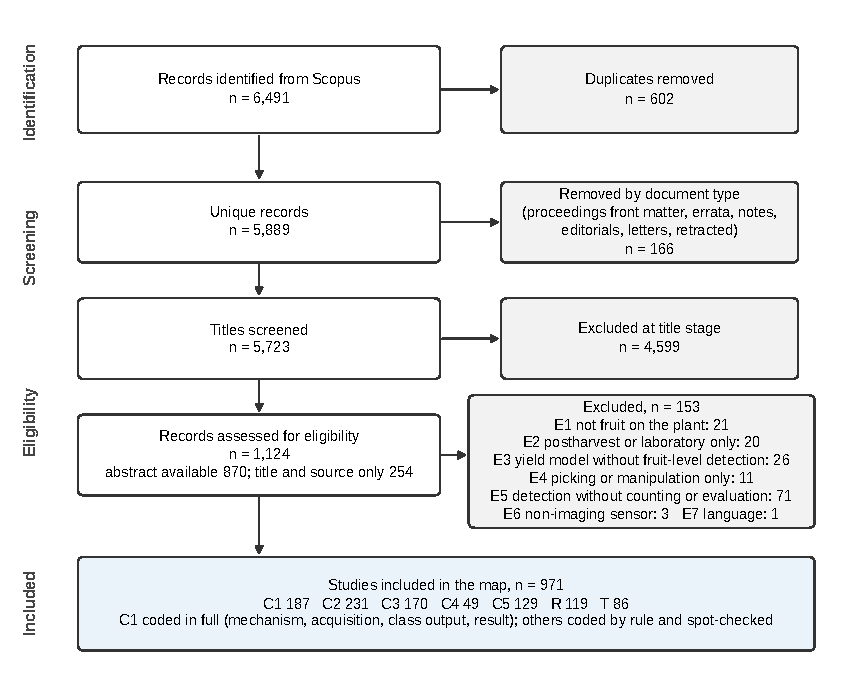
\includegraphics[width=0.78\textwidth]{F01_prisma}
\caption{PRISMA~2020 flow diagram of record identification, screening, eligibility assessment, and inclusion.}\label{fig:prisma}
\end{figure*}

\begin{figure*}[!t]
\centering
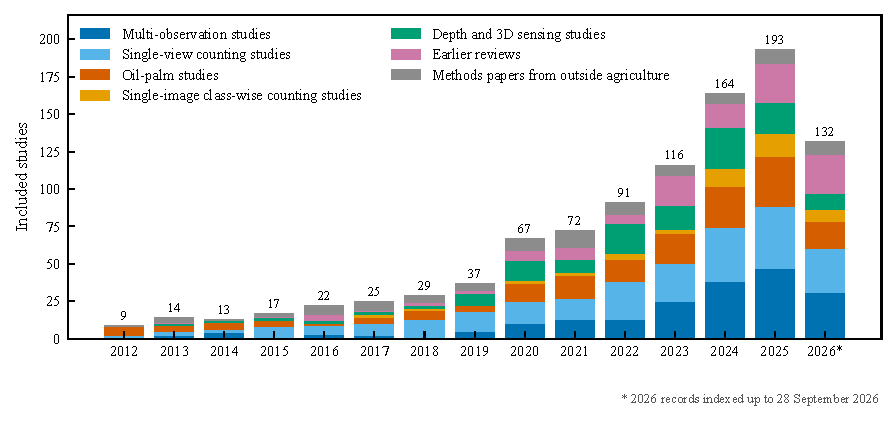
\includegraphics[width=0.85\textwidth]{F02_tahun}
\caption{Number of included studies per year by group ($n=\nScopusIncl$ studies identified through Scopus).}\label{fig:tahun}
\end{figure*}

Fig.~\ref{fig:terms} shows the term map: \nTerms terms and \nLinks links. Its three large clusters match the groups of the review: counting, yield estimation, video, and tracking sit together with the terms for identity (data association, re-identification, double counting, multi-view); depth, RGB-D, stereo, LiDAR, and point clouds sit with apple, orchard, occlusion, and localization; and ripeness, classification, and grading sit with oil palm. The identity terms are small and peripheral: each occurs in \nIdentTermMin to \nIdentTermMax of the \nScopusIncl studies, against \nTermDetection for detection and \nTermCounting for counting.

\begin{figure*}[!t]
\centering
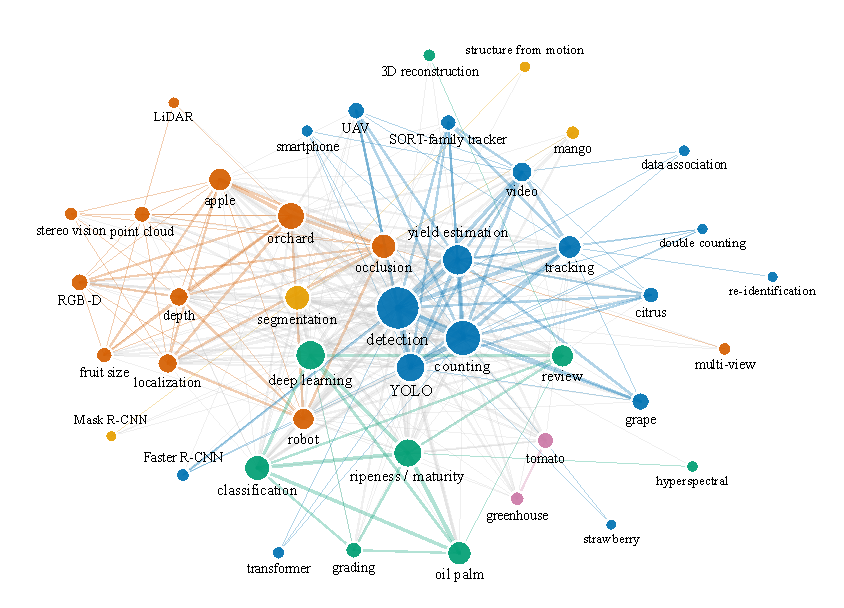
\includegraphics[width=0.82\textwidth]{F08_istilah}
\caption{Term co-occurrence map of the included studies, where node size, line width, and colour represent the number of studies containing the term in the title or abstract, the number of studies containing both terms, and the cluster, respectively.}\label{fig:terms}
\end{figure*}

\section{A design space for turning observations into records}\label{sec:framework}

This section (i) describes the five stages that lead from images to a class-wise inventory, (ii) names the ways in which a fruit is counted twice, (iii) defines the six association mechanisms by the condition each assumes, and (iv) reports how the \nMulti multi-observation studies are distributed over mechanisms, acquisition designs, crops, platforms, and sensors.

\subsection{From images to an inventory}
Fig.~\ref{fig:kerangka} shows the five stages of the pipeline that ends in a class-wise inventory. Acquisition fixes how many views of each plant exist, whether they are ordered in time, and whether pose, depth, or baseline are known. Observation produces detections or masks in each image; a fruit may produce several observations, and a detector may also split one fruit or merge two. Association decides which observations belong to the same physical fruit. Attribute assignment gives the unique fruit a class, size, or mass. The inventory aggregates unique fruit by class and by tree, row, or block. Detection accuracy, which most papers report, describes the second stage. The count, which the user needs, depends on all five.

\begin{figure*}[!t]
\centering
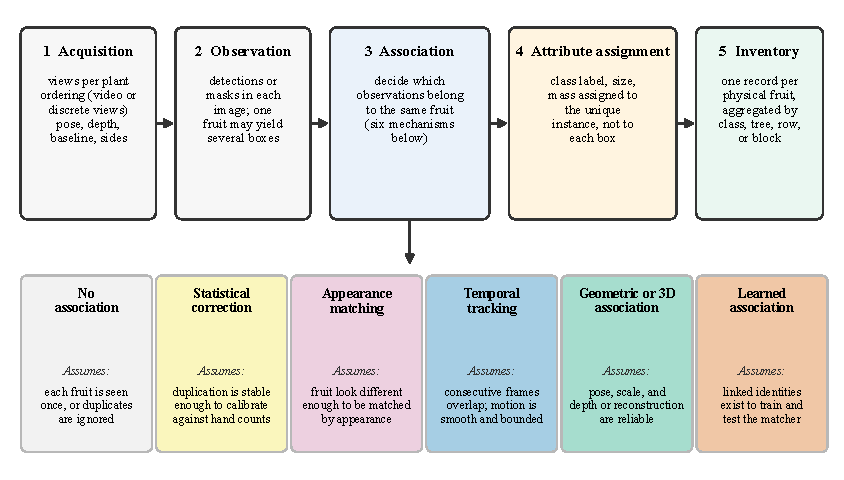
\includegraphics[width=0.92\textwidth]{F03_kerangka}
\caption{Design space: five stages from acquisition to inventory, and the six association mechanisms with the condition each assumes.}\label{fig:kerangka}
\end{figure*}

\subsection{Three sources of double counting}\label{sec:dupsources}
\citet{liu2019monocular} named three ways in which a fruit is counted twice in a traversal: the same fruit detected in consecutive images, the same fruit tracked, lost, and picked up again as a new track, and the same fruit seen from the two sides of a tree. \citet{wang2019mango} cited the same three sources when designing their mango tracker. Misses have two sources: fruit never visible from any camera position, and fruit visible but not detected. A mechanism controls some of these sources and not others, which is why the mechanisms below are described by what they assume, not only by how they compute.

\subsection{Six association mechanisms and the conditions they assume}\label{sec:mechdefs}
\textit{No association.} Each image is counted separately. This is correct only if acquisition guarantees that no fruit appears twice, or if duplicates are accepted.

\textit{Statistical correction.} Image counts are summed or averaged and then related to hand or harvest counts by a fitted factor or regression. No individual fruit is identified. It assumes that the ratio between observed and true counts is stable across the trees to which it is applied \citep{nuske2014modeling,linker2015estimation}.

\textit{Appearance matching.} Observations are linked when their appearance descriptors are similar, either hand-crafted or learned for re-identification. It assumes that fruit differ enough in appearance to be told apart.

\textit{Temporal tracking.} Observations in consecutive frames are linked by predicted motion and overlap, usually with a Kalman filter and an assignment step \citep{bewley2016simple}; a counting line or region then decides when a track is counted. It assumes that consecutive frames overlap and that motion between them is small and smooth.

\textit{Geometric or 3D association.} Observations are linked through a common coordinate frame: triangulation with known camera poses, structure from motion (SfM), simultaneous localization and mapping (SLAM), registered point clouds, or an implicit 3D representation such as a neural radiance field. It assumes that poses, scale, and depth or reconstruction are accurate enough that two different fruit are not placed at the same position.

\textit{Learned association.} A network is trained to decide correspondence directly from linked examples. It assumes that training data with identity links exist and represent the conditions of use.

A study may combine mechanisms; \nCombined of the \nMethod multi-observation method studies do (Appendix Table~\ref{tab:c1matrix}). In tables and figures a plus sign joins the mechanisms that a study combines, for example appearance + tracking. A study that combines them should still show which one removes the duplicates, because each fails under different conditions.

\subsection{Quantitative landscape of the multi-observation studies}\label{sec:landscape}
To complement the synthesis in Sections~\ref{sec:acq} to~\ref{sec:palm}, the coded records (Section~\ref{sec:coding}) were summarized with descriptive statistics. Of the \nMulti multi-observation studies, \nMultiData are dataset papers and \nMethod propose or evaluate a method; the statistics below refer to these \nMethod.

\textit{(i) Mechanisms and their change over time.} Fig.~\ref{fig:mek}(a) shows the share of method studies that use each mechanism in each period; because a study may combine mechanisms, the values are occurrences rather than mutually exclusive study counts. Temporal tracking appears in \nTrack of the \nMethod studies (\pTrack\%), geometric association in \nGeom (\pGeom\%), appearance matching in \nApp (\pApp\%), statistical correction in \nStat (\pStat\%), learned association in \nLearn, and no association in \nNone. The mix has shifted. Of the \nEarly studies published before 2018, \nEarlyGeom used geometric association, \nEarlyStat statistical correction, and \nEarlyTrack temporal tracking; since 2023, temporal tracking has appeared in \pTrackRecent\% of the \nRecent new studies and appearance matching, mostly inside trackers that carry an appearance descriptor, in \pAppRecent\%.

\textit{(ii) Acquisition design.} Fig.~\ref{fig:mek}(b) shows that most studies acquire video along a path (\nVideo); \nDiscrete use discrete views, \nScan use 3D scans, \nRevisit revisit the same plants over time, and \nSingleView is coded as a single view. The literature is therefore mainly a literature of video.

\textit{(iii) Crops and class reporting.} Fig.~\ref{fig:crop} relates crop to mechanism. Apple accounts for \nCropApple studies, citrus for \nCropCitrus, grape for \nCropGrape, tomato for \nCropTomato, strawberry for \nCropStrawberry, and mango for \nCropMango. Only \nPerClass of the \nMethod studies report counts per class, which Section~\ref{sec:class} takes up.

\begin{figure*}[!t]
\centering
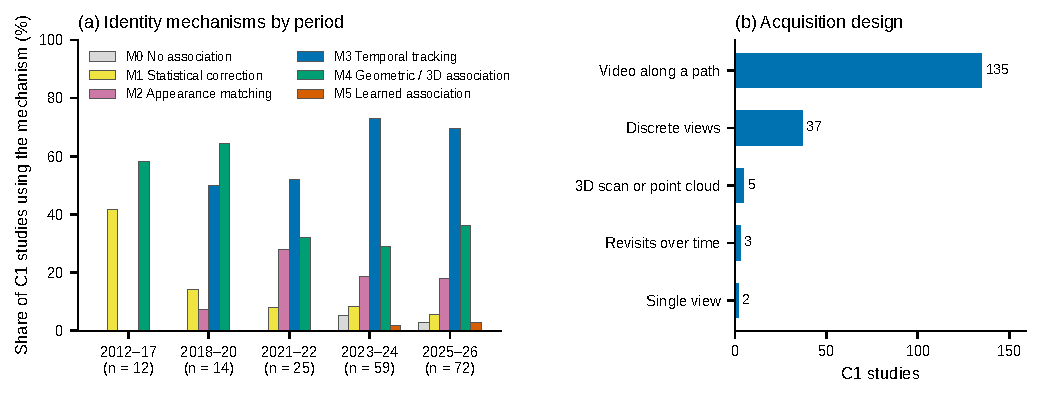
\includegraphics[width=0.9\textwidth]{F04_mekanisme}
\caption{Association mechanisms and acquisition design in the multi-observation method studies ($n=\nMethod$): (a) share of studies using each mechanism by period; (b) acquisition design.}\label{fig:mek}
\end{figure*}

\begin{figure*}[!t]
\centering
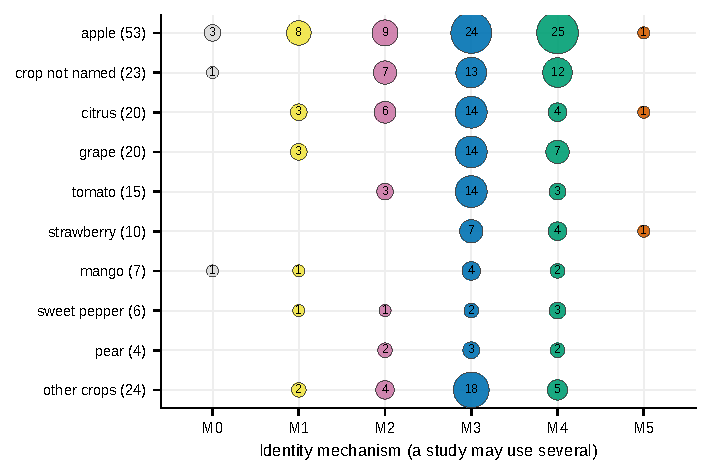
\includegraphics[width=0.6\textwidth]{F05_tanaman_mekanisme}
\caption{Multi-observation method studies by crop and association mechanism ($n=\nMethod$), where the number in each circle is the study count.}\label{fig:crop}
\end{figure*}

\textit{(iv) Combinations, from acquisition to crop.} Fig.~\ref{fig:flow} follows each of the \nMethod studies from acquisition to crop. Here a study is placed in one category, so combinations are separate: temporal tracking alone accounts for \nTrackOnly studies, geometric association alone for \nGeomOnly, appearance matching combined with temporal tracking for \nAppTrack, and temporal tracking combined with geometric association for \nTrackGeom. Video feeds all four of these, whereas discrete views lead mainly to geometric association (\nDiscreteGeom of the \nDiscrete studies) and to statistical correction (\nDiscreteStat). Taken together, Fig.~\ref{fig:mek}(a) counts every mechanism a study uses, whereas Fig.~\ref{fig:flow} places each study in one category; the first shows prevalence and the second shows which combinations occur.

\textit{(v) Platforms and sensors.} Fig.~\ref{fig:sensor} gives modality and platform by crop. The platform is the least reported property: \nPlatNone of the \nMethod abstracts do not state it, \nPlatGround name a ground vehicle or robot, \nPlatUav an unmanned aerial vehicle (UAV), \nPlatHand a handheld device or smartphone, and \nPlatSeveral name more than one platform; in Fig.~\ref{fig:sensor}(b) a study that names several platforms is counted under each. These counts describe what abstracts report, not what was used. An RGB camera is the sensor in \nModRgb of the \nMethod studies; RGB-D cameras appear in \nModRgbd, stereo cameras in \nModStereo, LiDAR in \nModLidar, and multispectral cameras in \nModMulti. Sensors that measure depth are concentrated in apple and strawberry.

\begin{figure*}[!t]
\centering
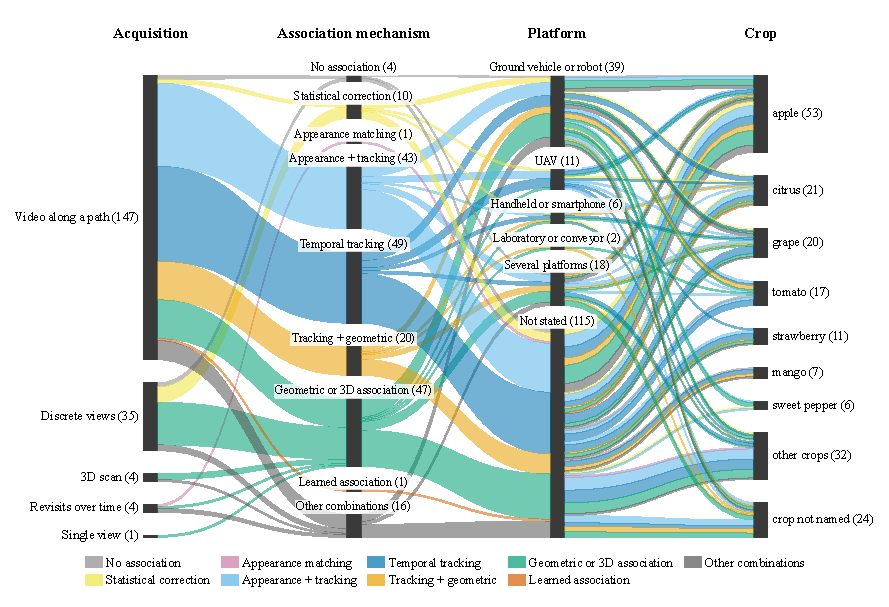
\includegraphics[width=0.92\textwidth]{F09_alur}
\caption{Acquisition design, association mechanism, platform, and crop of the multi-observation method studies ($n=\nMethod$), where band width and colour represent study count and mechanism, respectively.}\label{fig:flow}
\end{figure*}

\begin{figure*}[!t]
\centering
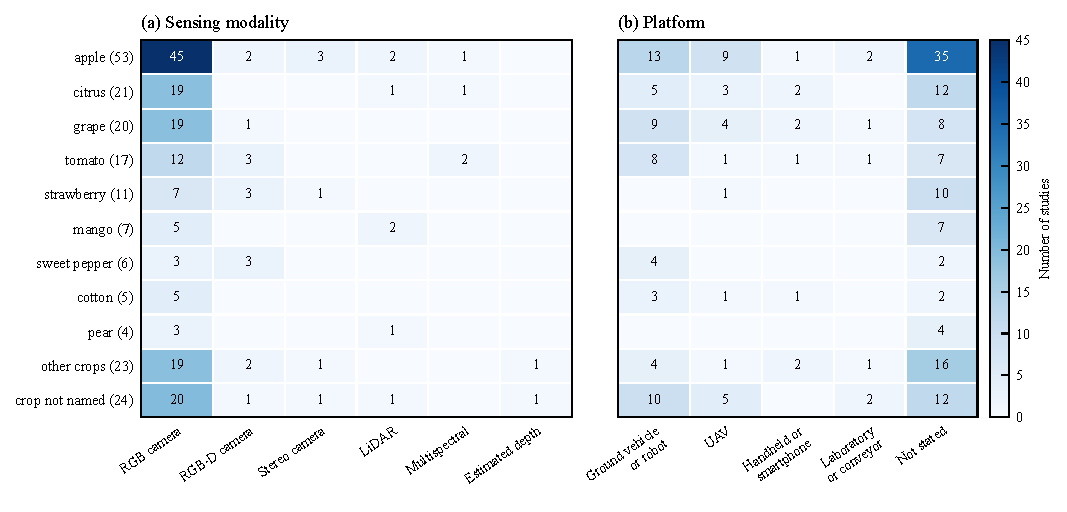
\includegraphics[width=0.9\textwidth]{F10_sensor}
\caption{Sensing modality and platform by crop in the multi-observation method studies ($n=\nMethod$): (a) modality; (b) platform.}\label{fig:sensor}
\end{figure*}

Sections~\ref{sec:acq} to~\ref{sec:palm} use this design space. Section~\ref{sec:acq} takes the acquisition stage, Section~\ref{sec:mech} the association stage one mechanism at a time, and Section~\ref{sec:class} the attribute stage; Sections~\ref{sec:depth} and~\ref{sec:palm} then ask what depth sensing and the oil-palm case add.

\section{Acquisition: how many views, and from where}\label{sec:acq}

This section covers the acquisition stage. Eight studies compared acquisition designs on the same plants (Table~\ref{tab:acq}); their results show how much recall additional views add and when they do not help. Each row is one study; the values are as reported and should be compared only within a row, because references and metrics differ between studies (Section~\ref{sec:mech-measure}).

\begin{table*}[!t]
\centering
\caption{Studies that compared acquisition designs on the same plants ($n=8$).}\label{tab:acq}
\footnotesize
\begin{tabularx}{\textwidth}{@{}L{2.6cm}L{1.6cm}L{2.9cm}YL{2.4cm}@{}}
\toprule
Study & Crop, scale & Designs compared & Reported result & Count reference\\
\midrule
\citet{stein2016image} & Mango, 16 trees & One image of one side; one image per side; multi-view tracking with triangulation (tracking + geometric) & Fruit counted: 27\% (single, $R^2=0.81$), 54\% (dual, $R^2=0.94$), 101.4\% (multi-view, $R^2=0.90$) & Hand count on tree and at harvest\\
\citet{wang2019mango} & Mango, 21 trees & One image per side; video tracking & 40\% of harvest (bias-corrected RMSE 21.7 fruit/tree) vs 62\% (RMSE 18.0) & Harvest count\\
\citet{gongal2016apple} & Apple, tall spindle & One side; both sides with 3D duplicate removal (geometric association) & Crop-load estimation accuracy 58\% vs 82\%; error in identifying duplicate apples 21.1\% & Manual count\\
\citet{qureshi2023seeing} & Apple fruitlets & One-sided vs two-sided scans from an over-canopy robot & Counting accuracy 73.7\% vs 81.17\% & Manual count\\
\citet{arizasentis2025comparative} & Grape, commercial vineyard & Single-view vs multiple-view UAV video with tracking & Tracked/ground-truth ratio 13--23\% vs 27--74\% across trials; multi-view tracking degraded by motion blur & Annotated video\\
\citet{felippomes2026video} & Apple, 420 trees & Two RGB-D sensors, three distances, two dates, one or both sides & Best MAPE 6.91\%, $R^2=0.733$ at 225~cm; both sides improved estimates per row stretch & Manual count\\
\citet{vijayakumar2023tree} & Citrus, per tree & UAV features plus fruit counts from one or two sides & MAPE 23.45\% (one side) vs 25.72\% (two sides), both better than UAV only (35.59\%) & Harvest per tree\\
\citet{anderson2021estimation} & Mango, 20 orchards & Raw multi-view counts vs multi-view corrected with hand counts & Absolute percentage error on packhouse count 11\% vs 17\% (nine orchards with all methods, 2019--2020 season); trellised canopies overestimated by 25.2\% against harvest counts & Packhouse count; harvest count (canopy trial)\\
\bottomrule
\multicolumn{5}{@{}p{\textwidth}@{}}{\rule{0pt}{2.6ex}\textit{Note:} Values are as reported by the authors. Count references and metrics differ between rows, so values should be compared only within a row. MAPE, mean absolute percentage error; RMSE, root-mean-square error; UAV, unmanned aerial vehicle.}
\end{tabularx}
\end{table*}

Three results are consistent across the eight comparisons.

\textit{(1) A single image per side sees a minority of the fruit on a dense canopy.} \citet{stein2016image} counted 27\% of the fruit from one side and 54\% from two sides of mango trees, and \citet{wang2019mango} counted 40\% of the harvest with one image per side. In apple, \citet{gongal2016apple} reached a crop-load estimation accuracy of 58\% with single-side imaging against 82\% with dual-side imaging.

\textit{(2) Low recall does not prevent a precise estimate if it is calibrated.} In the study of \citet{stein2016image}, the dual-view counts correlated with the true counts more tightly ($R^2=0.94$) than the multi-view counts ($R^2=0.90$), but they had to be scaled up by a factor near two. Precision and accuracy therefore answer different questions; a correlation with hand counts does not show that duplicates were removed.

\textit{(3) Adding views does not always help.} \citet{vijayakumar2023tree} found that counts from the second side did not reduce the per-tree yield error in citrus, whereas \citet{arizasentis2025comparative} recovered more bunches with multiple-view flights over a vineyard but lost tracking quality to motion blur. \citet{zhu2024citrus} found that the best number of views per citrus tree (two, four, or six) depended on how heavily the tree had been pruned. More views therefore raise recall but do not guarantee a lower error per tree.

\textit{How acquisition constrains association.} Acquisition also decides which association mechanisms are possible. Video along a row gives the frame-to-frame overlap that temporal tracking needs. Discrete views around a tree, as in SawitMVC \citep{indriani2026sawitmvc} or the eight direction frames that \citet{nenavath2024tree} sampled at equal intervals from a 360-degree walk-around video of a mango tree, have wide baselines and no frame-to-frame continuity, so tracking does not apply and association must rely on appearance, geometry, or learning. Several groups have treated view selection itself as the problem: active view planning for apple clusters \citep{roy2017active}, viewpoint planning with an octree of fruit regions \citep{zaenker2021viewpoint}, and graph-based view sequences for sweet pepper \citep{zaenker2023graph}. These studies optimize coverage; they do not report counts against a reference.

Taken together, the eight comparisons show that acquisition limits how much of the fruit can be seen and decides which association mechanisms can be applied; Section~\ref{sec:mech} examines those mechanisms.

\section{Evidence by association mechanism}\label{sec:mech}

This section addresses the first two questions for the association stage: which mechanism was used, and what evidence shows that it controls duplicates and misses. Temporal tracking appears in \nTrack of the \nMethod method studies and geometric association in \nGeom (Section~\ref{sec:landscape}), so these two subsections are the longest. The subsections run from the mechanisms that identify no individual fruit, to linking in the image by motion and by appearance, to linking in a common 3D frame, and to correspondence learned from linked examples. Table~\ref{tab:assoc} collects the 14 comparisons that were made on the same data; the values are as reported by the authors and can be compared within a row but not between rows. All studies coded for each mechanism are listed in Appendix Table~\ref{tab:c1matrix}.

\begin{table*}[!t]
\centering
\caption{Comparisons of association mechanisms on the same data ($n=14$).}\label{tab:assoc}
\footnotesize
\begin{tabularx}{\textwidth}{@{}L{2.8cm}L{1.7cm}L{3.4cm}YL{1.8cm}@{}}
\toprule
Study & Crop & Compared & Reported result & Metric level\\
\midrule
\citet{zhang2022deep} & Citrus & OrangeSort (motion, counting region) vs SORT vs DeepSORT & Counting MAE 0.081 vs 0.45 vs 1.212 & Count\\
\citet{genemola2023video} & Apple & ByteTrack vs SORT vs DeepSORT (YOLOv5x) & HOTA 0.689, 0.680, 0.682; DeepSORT 128~ms per image vs about 15~ms; MAPE 7.47\% one week before harvest & Identity and count\\
\citet{piazolo2026enhanced} & Grape (UAV) & SORT vs SORT+ with extended matching cascade & Counting accuracy 33\% to 96\%; ID switches $-62$\%; MOTA and IDF1 +5--6\% & Identity and count\\
\citet{poncemachete2025optimizing} & Calamansi (UAV) & SORT, DeepSORT, ByteTrack & ByteTrack best: MOTA 59.67\%, HOTA 65.42\%, IDF1 73.72\% & Identity\\
\citet{wei2025multi} & Apple (stereo) & OC-SORT vs ByteTrack with GPS and visual odometry & OC-SORT best (HOTA 0.59); total error 20 apples, RMSE 6.24\%, $R^2=0.96$ & Identity and count\\
\citet{qi2025assessment} & Tomato clusters & SORT, DeepSORT, ByteTrack, BoT-SORT at reduced frame rates & Public MOT dataset with 165{,}172 cluster instances & Identity\\
\citet{liu2018robust} & Orange, apple & Tracking alone vs tracking plus SfM correction (tracking vs tracking + geometric) & SfM step rejected double-counted tracks and outliers; L1 count error fell from 593 to 203 (orange) and from 673 to 322 (apple) & Count\\
\citet{hani2020comparative} & Apple, three datasets & Summed counts of the two sides vs counts merged in a 3D reconstruction of both sides (no association vs geometric) & 103.86--147.81\% vs 95.56--97.83\% of the harvested count & Count\\
\citet{genemola2020fruitb} & Apple, 11 trees & 2D detection vs detection projected into SfM (geometric) & F1 0.816 to 0.881 against 1{,}455 apples annotated in the 3D point cloud & Detection in 3D\\
\citet{genemola2020fruit} & Apple & LiDAR from one position vs multi-view, with and without forced air & 6.5\% (multi-view) and 6.7\% (air flow) more fruit located & Detection in 3D\\
\citet{lei2025spatio} & Apple, 60 trees (association ground truth: five trees) & 4D association (position, appearance, topology) vs position-only and histogram-descriptor baselines & Association precision +23.7\% over the descriptor baseline; counting accuracy 96.9\% (1{,}846 estimated vs 1{,}790 apples) & Identity and count\\
\citet{hong2025fruitgaussian} & Persimmon & 3D Gaussian splatting vs NeRF-based counting & Counting accuracy 96\%, reported as 16\% above NeRF-based methods & Count\\
\citet{xing2026lightweight} & Cherry tomato & Tracking with and without multi-view compensation & Counting error reduced by 95.6\% & Count\\
\citet{mollineda2025estimation} & Orange & Regression from single frames vs video segments & Multi-frame segments better, tested with nonparametric statistics & Count\\
\bottomrule
\multicolumn{5}{@{}p{\textwidth}@{}}{\rule{0pt}{2.6ex}\textit{Note:} Values are as reported by the authors and should be compared only within a row. Metric level: Count, agreement of the final count with a reference; Identity, tracking metrics such as multiple-object tracking accuracy (MOTA), the identification F1 score (IDF1), higher-order tracking accuracy (HOTA), or identity (ID) switches; Detection in 3D, detection F1 after projection. Metrics are given in the scale used by each paper (fraction or per cent). MAE, mean absolute error; MAPE, mean absolute percentage error; RMSE, root-mean-square error; SfM, structure from motion; NeRF, neural radiance field.}
\end{tabularx}
\end{table*}

\subsection{No association and statistical correction}\label{sec:mech-stat}
Statistical correction is used in \nStat of the \nMethod method studies (\pStat\%), and \nNone apply no association (Section~\ref{sec:landscape}). The studies without association rely on acquisition to limit duplicates. \citet{nenavath2024tree} summed the mangoes detected in eight direction frames of a tree and counted 133 fruit against a manual count of 130 on one tree, with a counting accuracy of 95.48\% on 14 trees. \citet{tureckova2022slicing} avoided tracking by stitching a narrow vertical strip of every video frame into one panorama of a tomato row and counting once in that image; the detected count differed from the annotated count by 2.32\%. \citet{villacres2024assessing} reported that one camera perpendicular to an apple canopy detected up to 88.3\% of the fruit detected by four cameras.

The earliest multi-image systems summed counts and calibrated them. \citet{nuske2014modeling} registered images from a vehicle driving along vineyard rows and related berry counts to harvest yield; with calibration data from a prior harvest the estimate was within 4\%, and within 3\% with destructive samples taken at the time of imaging. Across four seasons their estimates captured up to 75\% of the spatial variance in yield \citep{nuske2014automated}. \citet{linker2015estimation} photographed 42 apple trees from two sides at three heights, summed the six counts per tree, and calibrated the sum against 14 trees; the orchard estimate was within 10\% of the actual yield although single-tree errors were sometimes large. \citet{song2014automatic} aggregated repeated, incomplete observations of pepper fruit in over 28{,}000 images of more than 1{,}000 plants with a statistical clustering step and reached a correlation of 74.2\% with manual counts without linear adjustment.

The strength of statistical correction is repeatability. \citet{stein2016image} found the dual-view counts more tightly correlated with true counts than any other design, and \citet{anderson2021estimation} reported absolute errors of 2\% or less in repeated night-time imaging of mango orchards. The weakness is transfer. The factor describes an average tree and cannot say which fruit was counted twice. It must be refitted when canopy, cultivar, or acquisition changes. \citet{anderson2021estimation} found the error on trellised canopies (25.2\%) to be several times that on hedge, single-leader, or conventional systems (3.4--8.2\%), and in the 2019--2020 season, across the nine orchards with all methods, correcting multi-view counts with hand counts of a stratified sample increased the average error from 11\% to 17\%. Regression from partial views to total counts remains common in UAV work: \citet{apoloapolo2020cloud} related top-view apple counts to total counts per tree with $R^2=0.80$, and \citet{li2023blueberry} used a regression across three views to account for blueberries seen more than once.

Collectively, these studies show that statistical correction gives repeatable block-level estimates but no record of which fruit was counted twice; it is the baseline against which the other mechanisms should be tested (Section~\ref{sec:agenda}).

\subsection{Temporal tracking}\label{sec:mech-track}
Temporal tracking is the most common mechanism: it appears in \nTrack of the \nMethod method studies (\pTrack\%) and in \pTrackRecent\% of those published since 2023 (Fig.~\ref{fig:mek}a). Most studies follow tracking by detection: a detector finds fruit in each frame, a Kalman filter predicts where each track should appear next, and an assignment step, usually the Hungarian algorithm on overlap or distance, links detections to tracks \citep{bewley2016simple,wojke2017simple,zhang2022bytetrack}. Four issues recur in these studies.

\textit{(1) The counting rule.} A counting rule decides when a track becomes a fruit. Two rules dominate: count each unique track identity, or count a track when it crosses a line or region. \citet{parico2021real} found the unique-identity rule more reliable for pears (F1 87.85\%), because detection flicker caused the line rule to miss fruit that were detected, whereas \citet{zhang2022deep} counted citrus only when a track entered a fixed region, and this rule gave the lowest error in Table~\ref{tab:assoc}.

\textit{(2) Motion alone versus motion with appearance.} The main question within temporal tracking is whether appearance features help. In the two comparisons on the same apple and citrus data, DeepSORT, which adds a learned appearance descriptor to the motion model, did not outperform trackers that use motion alone \citep[Table~\ref{tab:assoc};][]{zhang2022deep,genemola2023video}. In the citrus study its counting error was higher than that of SORT (MAE 1.212 against 0.45) \citep{zhang2022deep}, and in the apple study it needed 128~ms per image against about 15~ms \citep{genemola2023video}. \citet{saraceni2024agrisort} designed AgriSORT to use motion only, arguing that fruit are static targets of similar appearance, and released a table-grape benchmark with strong self-similarity. \citet{piazolo2026enhanced} improved SORT with a matching cascade over Mahalanobis, intersection-over-union, and Euclidean distances and reached accuracy comparable to DeepSORT without identity training data. The same issue appears outside agriculture: DanceTrack was built because targets with uniform appearance and diverse motion defeat trackers that rely on appearance \citep{sun2022dancetrack}. Studies that reported good results with DeepSORT exist, for example banana bunches with RGB-D and three constraints (96.82\% counting success) \citep{zhou2025yield}, but they did not compare against a motion-only tracker on the same data.

\textit{(3) Repairs for broken tracks.} The failure modes that tracking studies report are specific. Missed detections break tracks and create new identities; \citet{zhang2025robust} added trajectory prediction to bridge such gaps in blueberry video, and \citet{zhou2024advancing} added a multiple-mapping step for occluded strawberries. Camera shake on a legged robot reduced tracking accuracy until camera-motion compensation added 2.9 points of MOTA \citep{zhang2024stablesort}, and low frame rates from UAVs motivated motion-direction costs and feature-based compensation in PineSORT \citep{xieli2025pinesort}. \citet{wang2019mango} measured the net effect in the most transparent way, by reporting double counts (9.9\%) and misses (7.3\%) separately instead of only their difference.

\textit{(4) What tracking does not resolve.} A fruit seen from both sides of a row appears in two separate passes. \citet{wang2019mango} listed it as a separate source of double counts, and \citet{liu2019monocular} used the depth of each fruit relative to its tree trunk to drop fruit that belong to the far side.

Taken together, these studies show that tracking links fruit across consecutive frames but cannot, by itself, resolve the third source of double counting (Section~\ref{sec:dupsources}); the studies that address it use geometric association (Section~\ref{sec:mech-geom}).

\subsection{Appearance matching}\label{sec:mech-app}
Appearance matching occurs in \nApp of the \nMethod method studies (\pApp\%), almost always together with another mechanism: \nAppTrack studies combine it with temporal tracking through trackers that carry an appearance descriptor, such as DeepSORT, StrongSORT, or BoT-SORT with its re-identification module (Section~\ref{sec:coding}). \citet{kirk2021robust} added a re-identification head to a multi-object tracker to count soft fruit through occlusions and reported a count error (MAPE) of 3\% against 21\% for a baseline tracker. \citet{xia2022culling} matched pairs of fruit patches between sequence images with a trained matching network and a one-to-one assignment, and reached F1 0.816 for apples and 0.864 for oranges in identifying repeated fruit. \citet{zheng2023object} combined image appearance and position in a learned distance (an improved FaceNet) and clustered strawberry fruit and flower detections from overlapping multi-view remote sensing images; the result recovered objects that the orthomosaic hid. The pattern across these studies is that appearance works when combined with motion or position and has not been shown to work as the only cue for look-alike fruit, which agrees with the tracker comparisons in Section~\ref{sec:mech-track} and with the person re-identification literature, where discriminative identity features are learned from large sets of labelled identities \citep{zheng2015scalable,ye2022deep}.

\subsection{Geometric or 3D association}\label{sec:mech-geom}
Geometric association is used in \nGeom of the \nMethod method studies (\pGeom\%); they are listed in Appendix Table~\ref{tab:c1matrix} and shown by crop in Fig.~\ref{fig:crop}. It is the route with the longest history of calibration-free counts. Five streams can be distinguished.

\textit{(1) Triangulation with poses from navigation sensors or stereo.} \citet{wang2013automated} used a stereo rig at night on an autonomous vehicle and registered sequential images; block-level errors were $-3.2$\% for about 480 red-apple trees and 1.2\% for about 670 green-apple trees. \citet{stein2016image} established pairwise correspondences between images from the trajectory of a navigation system, triangulated tracked fruit, and used LiDAR to assign each fruit to its tree; 522 trees and 71{,}609 mangoes were scanned and the error for individual trees was 1.36\%.

\textit{(2) Structure from motion from a single camera.} \citet{liu2018robust} replaced the navigation and LiDAR suite with a monocular camera: fruit were tracked in 2D and localized in 3D by structure from motion, and double-counted tracks were detected by their proximity in 3D. The later version also tracked trunks, built semantic structure-from-motion landmarks, and projected them back into every image \citep{liu2019monocular}. \citet{roy2016surveying} built a piecewise incremental SfM for apple rows because standard SfM failed under the constrained geometry of a row.

\textit{(3) Merging the two sides of a row.} \citet{roy2019vision} merged counts from both sides of the row on three validation datasets (6, 10, and 6 trees) with an accuracy of 91.98--94.81\% against harvested counts. \citet{hani2020comparative} reused this pipeline with a learned counting network and compared it with a plain sum of the two sides: the sum gave 103.86--147.81\% of the harvested count, and the merged reconstruction 95.56--97.83\% (Table~\ref{tab:assoc}). \citet{dong2020semantic} addressed the same two-side problem by aligning the reconstructions of both sides with global and semantic features, since the two sides share little overlap. \citet{gongal2016apple} used 3D positions to remove apples seen from both sides, but misidentified 21.1\% of duplicates.

\textit{(4) Counting in a 3D map.} Newer geometric systems move the whole count into 3D. \citet{genemola2020fruitb} projected Mask R-CNN detections into an SfM point cloud and improved F1 from 0.816 to 0.881, at a processing cost they judged unsuitable for real time. \citet{matos2024tracking} combined SfM with bipartite graph matching for apples filmed with unconstrained camera motion and low frame rates. \citet{lee2026lidarcamera} fused YOLO detections with SLAM point clouds from LiDAR in a 6~m by 70~m pear plot and reached 96.2\% counting accuracy. \citet{nellithimaru2019rols} built object-level SLAM from stereo for grape counting (F1 0.977 against image counts). \citet{rapadorincon2023development} tracked partial point clouds of tomatoes in 3D and estimated the total count with a best-case counting error of 5.06\%; they also showed that the final count of a tracker can hide false positives and false negatives that offset each other, and they introduced tracking metrics to expose them.

\textit{(5) Implicit representations.} FruitNeRF trains a semantic neural radiance field from posed images and clusters the extracted fruit points \citep{meyer2024fruitnerf}, and Gaussian splatting was reported to count persimmons with 96\% accuracy, 16\% above NeRF-based counting \citep{hong2025fruitgaussian}. These methods build on general reconstruction tools \citep{schonberger2016structure,mildenhall2020nerf,kerbl20233d}; their evaluations are still dominated by synthetic scenes and a few real trees.

\textit{Where geometry fails.} Scale is undefined for monocular reconstruction unless another sensor fixes it. Pose drift, where it occurs, enlarges the region within which two observations are declared the same fruit, so dense clusters can merge; no included study quantified this effect. Foliage moves between views, which violates the static-scene assumption of standard SfM and SLAM; dynamic-scene methods exist \citep{bescos2021dynaslam,saputra2019visual}, but no included fruit study measured how much foliage motion degrades counts. Assigning fruit to trees is a separate geometric problem; \citet{zineelabidine2021assigning} solved it by aligning a harvest-time point cloud to a leaf-off winter cloud in which each tree's branches are visible (accuracy above 95\%).

Overall, geometric association has produced counts close to the reference without a fitted factor when pose, scale, and depth are reliable; the evidence for implicit representations still rests on synthetic scenes and a few real trees.

\subsection{Learned association}\label{sec:mech-learn}
A learned component decides the correspondence in \nLearn of the \nMethod method studies (Section~\ref{sec:landscape}), in three ways. First, a network matches fruit between scans or images. \citet{fusaro2026horticultural} segmented fruit in coloured point clouds (terrestrial laser scans of strawberries and photogrammetric reconstructions of apples), extracted a descriptor per fruit with a sparse convolutional network, and matched fruit between sessions with an attention-based network and a probabilistic assignment, the matching being evaluated on the strawberry data only. The matching network of \citet{xia2022culling} and the learned distance of \citet{zheng2023object}, discussed under appearance matching (Section~\ref{sec:mech-app}), belong to the same group. Second, a network learns identity inside a 3D representation. FruitNeRF++ lifts 2D instance masks that are inconsistent between views into 3D through instance embeddings trained with a contrastive loss; on a real apple set it reached F1 0.765, below the 0.881 of the fruit-specific method of \citet{genemola2020fruitb} \citep{meyer2025fruitnerf}. \citet{zhao2026adapting} combined cross-view contrastive learning with voting in a 3D Gaussian representation and reported F1 above 0.97 for plum and mango scenes with dense occlusion. Third, a network replaces the association step of a tracker or fuses the views directly. \citet{santos2026multi} used a learned point tracker for data association in orange video; on seven sequences the count was 978 against 879 annotated fruit (an error of 11.26\%), which did not improve on the authors' earlier pipeline. \citet{isobe2025mandarin} fused features from different angles of a 360-degree mandarin video in a transformer and regressed the count, without an explicit identity for each fruit.

Outside agriculture, learned association is established for tracking of people and vehicles, within a single camera on pedestrian benchmarks \citep{braso2020learning} and across cameras, where datasets with identities across cameras exist \citep{ristani2016performance,chavdarova2018wildtrack,tang2019cityflow}. The obstacle in fruit is the same one these datasets removed: learned association needs identity labels across views, and in the included corpus only a handful of fruit datasets provide them, among them GrapeMOTS \citep{arizasentis2024grapemots}, the tomato MOT set of \citet{qi2025assessment}, the 4D orchard set of \citet{lei2025spatio}, and SawitMVC \citep{indriani2026sawitmvc}. This limit is taken up in Section~\ref{sec:agenda}.

\subsection{How the evidence was measured}\label{sec:mech-measure}
Of the \nMethodAbs multi-observation method studies with an abstract, \nMetCount (\pMetCount\%) report agreement between estimated and reference counts, \nMetDet (\pMetDet\%) report detection quality, \nMetIdent (\pMetIdent\%) report an identity metric such as multiple-object tracking accuracy (MOTA), the identification F1 score (IDF1), higher-order tracking accuracy (HOTA), or identity (ID) switches, and \nMetNone (\pMetNone\%) report no quantitative metric in the abstract (Fig.~\ref{fig:metrik}). Identity metrics were developed for this purpose: HOTA balances detection and association accuracy \citep{luiten2021hota}, and IDF1 was designed for identities that persist across cameras \citep{ristani2016performance}. A count error alone cannot separate a correct count from offsetting duplicates and misses \citep{rapadorincon2023development,wang2019mango}.

The reference also varies. Hand counts on the tree measure what the camera could have seen, harvest and packhouse counts include fruit hidden from every view, and annotated images measure only what an annotator saw. In the coded records, the count reference is annotated images or video in \nRefAnnot of the \nMethod method studies, a hand count on the plant in \nRefTree, a harvest count in \nRefHarvest, and a packhouse count in \nRefPack; \nRefNone state no count reference in the source that was read (a study may use more than one). Results from different references are not comparable, which is why Tables~\ref{tab:acq} and~\ref{tab:assoc} report the reference or metric level for every row.

\begin{figure*}[!t]
\centering
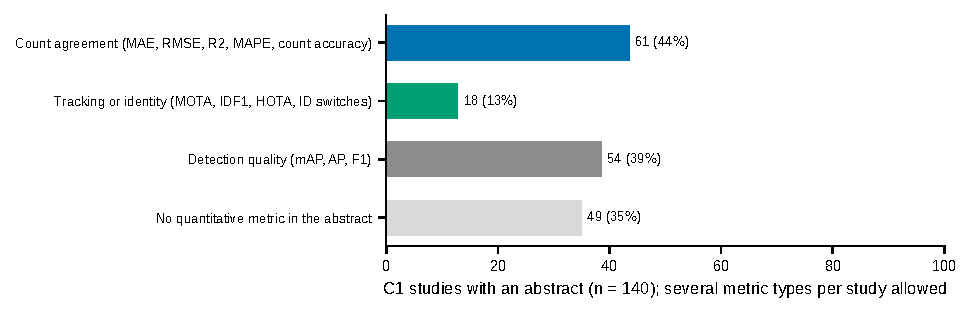
\includegraphics[width=0.62\textwidth]{F07_metrik}
\caption{Metric types reported in the abstracts of multi-observation method studies ($n=\nMethodAbs$).}\label{fig:metrik}
\end{figure*}

In answer to the first two questions, the included studies use six mechanisms whose assumptions are met by different acquisition designs (Section~\ref{sec:acq}), and the evidence that a mechanism controls duplicates and misses rests mostly on count agreement: 14 comparisons were made on the same data (Table~\ref{tab:assoc}) and \nMetIdent of the \nMethodAbs abstracts report an identity metric. Section~\ref{sec:agenda} turns these observations into gaps.

\section{Class attributes on unique fruit}\label{sec:class}

This section covers the attribute-assignment stage and answers the third question: how class attributes, mainly maturity, are attached to a unique fruit rather than to each detection. Two bodies of evidence bear on this.

\textit{Classes counted in single images.} The first is the \nClassSingle studies that detect and count fruit by class in single images. Most concern tomato (\nClassSingleTomato) and blueberry (\nClassSingleBlueberry), and \nClassSingleMaturity of the \nClassSingle use maturity as the class. \citet{maceachern2023detection} detected green, red, and blue wild blueberries with YOLOv4 and predicted yield by regression from the counts, whereas \citet{ni2020deep} counted blueberries with $R^2=0.886$ against ground truth. \citet{deng2024detection} released 17{,}955 annotated ripe and unripe blueberries in canopy images, and \citet{shimomoto2025predicting} predicted sweet pepper yield from average counts at two ripeness stages. These studies count classes in the image, not classes of unique fruit.

\textit{Class assigned during tracking.} The second is the \nPerClass multi-observation studies that report counts per class. Where the source states how the class is attached, it is most often carried by the tracker (\nClassDuring studies). \citet{ogundele2025real} used a class-aware ByteTrack for strawberries; counts correlated with ground truth at $R^2=0.914$ overall and at $R^2=0.950$ for ripe fruit. \citet{zhou2024advancing} reported a relative counting error of 6.7\%, with 8.7\% for ripe and 9.9\% for unripe strawberries. \citet{wang2025tomato} counted tomatoes in a counting region with ByteTrack and obtained a mean counting error of 6.6\% for all fruit but 12.3\%, 16.9\%, and 17.3\% for the ripe, half-ripe, and unripe classes. \citet{zheng2025robust} counted ripe tomatoes with an accuracy of 92.03--93.22\% and unripe tomatoes with 89.74--92.55\% against manual counts on three beds.

\textit{Class assigned after tracking or by a vote.} One study classifies after tracking \citep{pai2024maturity} and one resolves disagreement between frames explicitly: \citet{lin2026tomato} tracked tomatoes with StrongSORT and gave each tracked fruit the maturity class that received the most votes over its track. \citet{pardobeainy2026maturity} assigned each tracked strawberry to one of nine size--maturity categories from metric length and width derived from RGB-D point clouds and a colour-based ripeness percentage, and georeferenced the fruit with a global navigation satellite system for yield maps. \citet{wu2025maturity} reached an average counting accuracy of 72.49\% across blue, purple, and green blueberries in video. Other studies classify each tracked fruit but report only a total count: \citet{hassan2025orange} tracked oranges with ByteTrack and classified each tracked fruit as ripe or unripe with a separate network, and \citet{viveros2024maturity} tracked sweet peppers of four colours with YOLOv5 and DeepSORT and reported 85.7\% counting accuracy (MOTA 0.88 and 0.87) in two simulated environments, each a video assembled from 70 still greenhouse images.

\textit{Two consequences.} Two properties of class-wise counting follow from these results. First, class errors and identity errors interact. A fruit seen in ten frames can receive different labels in different frames, especially near class boundaries, and a class-aware tracker that splits the track when the label changes creates a duplicate. Only \nClassVote of the \nPerClass studies states a rule for choosing the label when frames disagree, \nClassUnstated do not state how the class is attached, and none of their abstracts reports a class confusion matrix computed on unique fruit. Second, per-class errors differ from the overall error. In the strawberry study of \citet{ogundele2025real} the ripe class had the highest count $R^2$ (0.950) and the lowest MAE (2.65 fruit), though not the lowest MAPE (11.63\% against 9.62\% for unripe), and in the tomato study of \citet{wang2025tomato} each class error was about twice the error for all fruit. In oil palm a video-based detector reached a mean average precision of 90.56\% for a single class but 70.21\% for several ripeness classes \citep{junior2023video}. An inventory that reports only a total hides both effects (Section~\ref{sec:agenda}).

\section{Depth and other modalities}\label{sec:depth}

Depth is examined separately because it can serve two stages of the design space: observation (finding, locating, and sizing a fruit) and association (placing observations in a common frame). The \nDepth depth and 3D sensing studies use RGB-D cameras (\nDepthRgbd), stereo (\nDepthStereo), LiDAR (\nDepthLidar), or other non-RGB signals. Their main use is not association but detection, localization, and sizing of individual fruit, most often apples (\nDepthApple). Four uses recur.

\textit{(1) Background removal.} \citet{fu2020faster} filtered objects farther than 1.2~m from a Kinect~V2 in a dense fruiting-wall orchard before detection.

\textit{(2) Fusion inside the detector.} \citet{tu2020passion} trained separate colour and depth detectors for passion fruit and fused them late, raising F1 from 0.885 for a standard Faster R-CNN on RGB-D images to 0.946. \citet{kaukab2024improving} filled depth holes before fusion because outdoor depth images are of low quality.

\textit{(3) Metric size.} \citet{wang2017tree} estimated on-tree mango dimensions from RGB-D with root-mean-square errors of about 4--5~mm but noted that the camera could not be used in direct intense sunshine. \citet{neupane2021evaluation} compared eight depth cameras against a 20~mm bias-corrected error requirement for fruit localization and sizing.

\textit{(4) Other active sensing.} LiDAR detected apples by reflectance with F1 0.858 \citep{genemola2019fruit}, and LiDAR--camera fusion reduced localization error to one fifth of that of a RealSense D455 \citep{kang2022accurate}. Active thermal imaging with water mist separated immature citrus from leaves of similar colour and supported tracking-based counting in video \citep{gan2020active}.

\textit{Depth for association.} For association, depth enters through geometric association (Section~\ref{sec:mech-geom}). \citet{zheng2025robust} filtered detections by depth and fused robot odometry before inter-frame prediction for tomatoes, reaching MOTA 0.954 against YOLOv8 with DeepSORT. \citet{abeyrathna2023recognition} obtained 3D coordinates of each tracked apple from a RealSense D455 at three vehicle speeds and three camera angles. \citet{felippomes2026video} found that the Azure Kinect gave more consistent results than the ZED~2 across dates in a 420-tree orchard. \citet{liu2019monocular} used depth relative to the trunk to resolve two-side duplicates. Monocular depth networks now offer depth without a depth sensor \citep{yang2024depthb,ranftl2021vision}, and one included study used such a network with amodal masks to measure apple diameter \citep{tan2025apple}, but none used predicted depth for cross-view association with a counted reference. The evidence therefore supports depth as an aid to separating neighbouring fruit and to placing fruit in a common frame when its error is small relative to fruit spacing, and it identifies the conditions (sunlight, range, registration) under which that error grows. Section~\ref{sec:palm} returns to these conditions for oil palm.

\section{Oil palm}\label{sec:palm}

This section answers the fourth question: what the oil-palm imaging literature covers, and what is missing for a bunch-level, class-wise census from images. It covers ripeness classification, detection, counting, and what the case implies for the choice of mechanism. Fig.~\ref{fig:sawit} shows that the \nPalm oil-palm studies concentrate on ripeness: \nPalmCls classify the ripeness of images of single bunches, \nPalmDet detect bunches in a scene, \nPalmSensor study non-RGB sensing of ripeness, \nPalmQual address quality, defects, mass, or pose, \nPalmLoose detect loose fruit, \nPalmCount count bunches, and \nPalmData are dataset papers. The setting is on the palm in \nPalmOnTree studies, at a mill, conveyor, or laboratory in \nPalmMill, on the ground or at a collection point in \nPalmGround, and from a UAV in \nPalmUav; \nPalmUnstated sources do not state it. Class labels are attached to instances in \nPalmInstClass studies. Only \nPalmViews use more than one view of the same bunch or palm.

\begin{figure*}[!t]
\centering
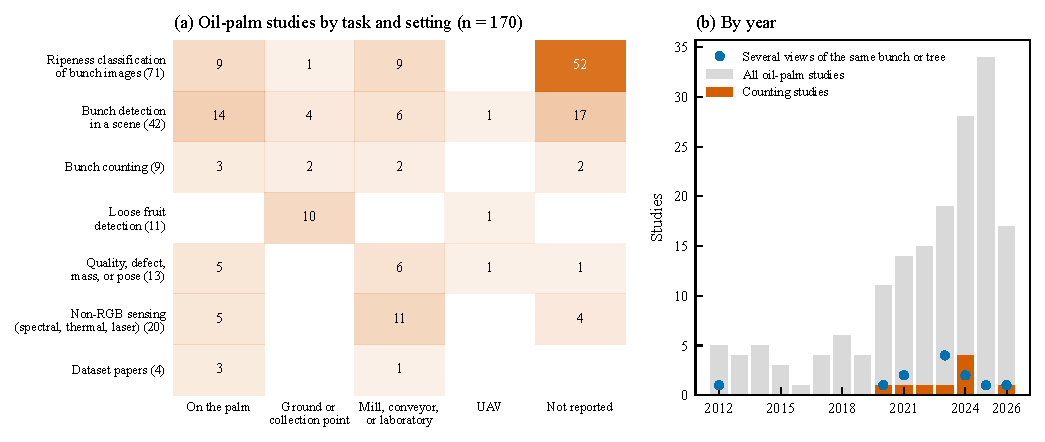
\includegraphics[width=0.9\textwidth]{F06_sawit}
\caption{Oil-palm studies ($n=\nPalm$): (a) task by setting; (b) studies per year, with counting studies and studies that use several views marked.}\label{fig:sawit}
\end{figure*}

\subsection{Ripeness classification and non-RGB sensing}
Ripeness classification has a long record. Early work extracted colour features and classified them with neural networks or support vector machines \citep{fadilah2012oil,sabri2018evaluation}, followed by colour and texture features classified with a back-propagation neural network \citep{septiarini2021machine} and by convolutional networks deployed on mobile devices \citep{suharjito2021oil}. The largest study in the corpus used 10{,}000 photographs from five Indonesian plantation sites in four classes and reported 94.66\% $\pm$ 0.54\% accuracy in leave-site-out cross-validation on sites not seen in training \citep{usman2026integration}. Reviews of this work agree that computer vision with deep learning is the most feasible field method \citep{lai2023oil} and that fusion with LiDAR may add localization \citep{goh2025fresh}. Non-RGB sensing has been tested with thermal imaging \citep{zolfagharnassab2022classification}, hyperspectral imaging \citep{bensaeed2014oil}, laser-light backscattering \citep{mohd2020combination}, LiDAR \citep{husin2021distribution}, and radar with bunch mass \citep{resta2026multimodal}, several of them on harvested bunches.

\subsection{Detection on the palm and at the mill}
Detection on the palm moved from single-class to multi-class ripeness detectors. \citet{lai2022real} trained YOLOv4 on images from a RealSense D435 with expert labels for ripe and unripe bunches, and \citet{mansour2022object} compared detectors on four ripeness classes. \citet{junos2021optimized} detected bunches, grabbers, and palms in plantation scenes, and the same group detected loose fruit in UAV images \citep{junos2022automatic}. \citet{zaman2025hybrid} addressed occlusion by fronds in UAV images. \citet{goh2025outdoor} released 400 plantation images with registered depth maps and point clouds from a RealSense D455f for ripeness classification and localization, the only oil-palm RGB-D dataset in the corpus. At the mill, \citet{suharjito2023real} graded piles of bunches from smartphone video and released annotated datasets of piles \citep{suharjito2023annotated}. Detection in oil palm therefore has field data, class labels, and one depth dataset, but each image is evaluated on its own.

\subsection{Counting}
Counting is the gap. The \nPalmCount counting studies count bunches in single images taken in the plantation \citep{naftali2024palm,hamdani2026automated,hidayat2024establishing,prasetyo2020automatic,hutapea2024palm}, count moving bunches on a laboratory conveyor with a colour-based detector and a centroid tracker \citep{shiddiq2023counting}, count unstripped bunches in a mill with Faster R-CNN and a Euclidean-distance tracker \citep{aji2021automatic}, count bunches and loose fruit together for harvest management \citep{daud2022loose}, or describe a counting system based on connected sensors \citep{narendran2024palm}. \citet{naftali2024palm} built a plantation dataset of video frames with partial visibility, occlusion, small objects, low contrast, and blur, \citet{hamdani2026automated} built a further plantation dataset, and \citet{hidayat2024establishing} proposed a standard procedure for capturing bunch images in the plantation.

None of the counting studies associates bunches across images of the same palm. \citet{suharjito2025oil} recorded unharvested palms from multiple angles with a smartphone for a digital census and released 14{,}503 images in five maturity classes, but the annotations are per image. The only oil-palm dataset in the corpus with cross-view identity links is SawitMVC, whose technical validation reports statistical baselines only: a regression from per-view counts placed 96.81\% of the per-class counts within one bunch of the reference when it was given the annotated boxes and 75.35\% when it was given detections \citep{indriani2026sawitmvc}. \citet{warni2026stereo} combined stereo detection with Hungarian matching to localize loose fruit in 3D, which is an association step, but for a stereo pair, not for views around a palm. Tree-level counting from UAV images has addressed re-counting errors for palms themselves \citep{pragatheesh2025deep,kipli2023deep}, not for bunches.

\subsection{Implications for the choice of mechanism}
The oil-palm case differs from the orchard cases in ways that matter for mechanism choice. Bunches of the same class on one palm look alike, which weakens appearance matching (Section~\ref{sec:mech-app}). A census photographs a palm from a few discrete positions, which removes the frame-to-frame continuity that temporal tracking needs (Section~\ref{sec:mech-track}). Fronds occlude bunches differently from each side, and the canopy is tall, which makes depth from consumer RGB-D cameras less reliable at the required range (Section~\ref{sec:depth}). The census classes are defined by months to harvest, so neighbouring classes differ in subtle colour changes, and a class error on one view can split one bunch into two records of different classes (Section~\ref{sec:class}). These four properties define the missing experiment that Section~\ref{sec:agenda} takes up.

\section{Position relative to earlier reviews}\label{sec:position}

With the evidence laid out, this section returns to the earlier reviews named in the Introduction and states what this review adds to each line of work. Table~\ref{tab:position} lists the earlier reviews that are closest to this one. The column ``Stated method'' records what each review states about how its studies were found, from the abstract or, where it was read, from the full text. Three reviews are organized by sensor or sensing technique \citep{gongal2015sensors,fu2020application,goh2025fresh}, three by method, architecture, or model type \citep{koirala2019deepb,maheswari2021intelligent,pu2025bridging}, three by estimation route, data source, or input feature \citep{anderson2021technologies,rong2026research,liu2026shaping}, and two oil-palm reviews by task or classifier \citep{khan2021oil,lai2023oil}. Reviews of tracking and re-identification outside agriculture \citep{luo2021multiple,rakai2022data,ye2022deep} and of 3D reconstruction \citep{saputra2019visual,zheng2026feed} provide the mechanisms but not the agricultural evidence.

\begin{table*}[!t]
\centering
\caption{Earlier reviews closest to this review ($n=11$).}\label{tab:position}
\footnotesize
\begin{tabularx}{\textwidth}{@{}L{3.1cm}YL{3.6cm}L{3.6cm}@{}}
\toprule
Review & Scope & Organizing variable & Stated method\\
\midrule
\citet{gongal2015sensors} & Fruit detection and localization for harvesting and crop-load estimation in apples, pears, citrus & Sensor and system & Not stated\\
\citet{koirala2019deepb} & Deep learning for fruit detection and yield estimation; extrapolation of image counts for occluded fruit & Method and application & Not stated\\
\citet{fu2020application} & Consumer RGB-D cameras for fruit detection and localization & Depth principle and sensor & Not stated\\
\citet{anderson2021technologies} & Forecasting fruit load and harvest timing & Estimation route (sampling, vision, remote sensing, models) & Not stated\\
\citet{maheswari2021intelligent} & Semantic segmentation for fruit yield estimation & Network architecture & Not stated\\
\citet{khan2021oil} & Machine learning in oil palm, 2011--2020 & Task (regression, classification) & Systematic, 61 papers\\
\citet{lai2023oil} & Oil-palm fresh-fruit-bunch ripeness detection & Sensing modality and classifier & Systematic, 51 papers\\
\citet{goh2025fresh} & Fresh-fruit-bunch ripeness classification & Sensing technique & Self-described systematic; no databases or search strings reported\\
\citet{pu2025bridging} & UAV counting of field crops & Agronomic target and model type & 52 key studies\\
\citet{rong2026research} & Orchard yield estimation with multi-source sensing & Data source & PRISMA\\
\citet{liu2026shaping} & Citrus yield prediction: input features, acquisition platforms and feature extraction, prediction models, and related estimation, monitoring, and measurement methods & Input feature, acquisition platform, and prediction model & Self-described systematic; search details not given in the abstract\\
\midrule
This review & Turning repeated fruit observations into unique, class-labelled records; oil palm as the main case & Association mechanism and its assumptions & Systematic map, Scopus, \nIncluded studies\\
\bottomrule
\multicolumn{4}{@{}p{\textwidth}@{}}{\rule{0pt}{2.6ex}\textit{Note:} None of the earlier reviews uses identity across observations as its organizing variable. Not stated: the abstract does not state how studies were found. PRISMA, Preferred Reporting Items for Systematic Reviews and Meta-Analyses; UAV, unmanned aerial vehicle.}
\end{tabularx}
\end{table*}

None of these reviews organizes the evidence by identity across observations, although several discuss occlusion and extrapolation from partial counts; the gaps that follow from doing so are set out in Section~\ref{sec:agenda}.

\section{Gaps and a measurement agenda}\label{sec:agenda}

This section synthesizes Sections~\ref{sec:acq} to~\ref{sec:palm}. Rather than repeating individual studies, it first traces how the choice of mechanism has shifted, then answers the four questions, and then states five gaps, each tied to the measurement that would close it.

\subsection{How the choice of mechanism has shifted}
Before 2018, geometric association and statistical correction accounted for almost all multi-observation studies; since 2023, temporal tracking has appeared in \pTrackRecent\% of new studies (Fig.~\ref{fig:mek}a). Within geometric association, implicit 3D representations are the latest variant, and \nLearn studies learn part of the association (Sections~\ref{sec:mech-geom} and~\ref{sec:mech-learn}). The trajectory therefore runs from correcting a sum, to linking detections in video, to placing fruit in a 3D frame. Class-wise identity has not followed: only \nPerClass of the \nMethod method studies report counts per class (Section~\ref{sec:class}). The term map agrees: each identity term occurs in \nIdentTermMin to \nIdentTermMax of the \nScopusIncl studies (Fig.~\ref{fig:terms}).

\subsection{Answers to the four questions}
\textit{Which mechanisms have been used, and what does each assume?} Six mechanisms are in use (Section~\ref{sec:mechdefs}). Temporal tracking assumes overlapping, ordered frames and is therefore tied to video; geometric association assumes reliable pose, scale, and depth; appearance matching assumes fruit that can be told apart; statistical correction assumes a stable ratio between observed and true counts; and learned association assumes identity-labelled data (Sections~\ref{sec:acq} and~\ref{sec:mech}).

\textit{How well does each mechanism control duplicates and misses, and how was that measured?} The evidence is mostly count agreement against references that differ between studies (Section~\ref{sec:mech-measure}). The 14 comparisons on the same data show that motion-only trackers were not outperformed by trackers with appearance features on look-alike fruit, and that a geometric step removed duplicates that tracking or summation left (Table~\ref{tab:assoc}).

\textit{How are classes attached to unique fruit?} In the \nPerClass studies that report counts per class, the class is mostly carried by the tracker; one study states a voting rule for disagreeing frames (Section~\ref{sec:class}).

\textit{What does the oil-palm literature cover, and what is missing?} It covers ripeness classification, detection, and counting in single images or on conveyors. No study associates bunches across views of a palm, and the one dataset with cross-view identity links has been evaluated with statistical baselines only (Section~\ref{sec:palm}).

\subsection{Five gaps}
\textit{(i) Identity is rarely measured.} Only \nMetIdent of the \nMethodAbs multi-observation method studies with an abstract (\pMetIdent\%) report an identity metric (Section~\ref{sec:mech-measure}, Fig.~\ref{fig:metrik}). A study that claims to remove duplicates should report, on annotated sequences or view sets, the numbers of duplicate records, missed fruit, false merges of two fruit into one, and identity switches, in addition to the count error. \citet{wang2019mango} and \citet{rapadorincon2023development} show that this is feasible.

\textit{(ii) Mechanisms are rarely compared on the same data.} Table~\ref{tab:assoc} contains 14 such comparisons, most within temporal tracking. Comparisons across mechanisms, for example tracking against geometric association on the same trees, are rare, and comparisons against a calibrated statistical-correction baseline are rarer, although image counts can be corrected to total fruit load with an occlusion factor regressed against manual counts of a set of calibration trees in each orchard \citep{koirala2019deepb,anderson2021technologies}. A new mechanism should be tested against a statistical correction fitted on separate trees.

\textit{(iii) Class-wise identity is almost absent.} \nPerClass multi-observation studies report counts per class, and one states how label disagreement between frames is resolved (Section~\ref{sec:class}). The required measurement is a per-class count error computed on unique fruit, together with a confusion matrix of classes on unique fruit.

\textit{(iv) Discrete-view protocols lack mechanisms.} Most methods assume video (Fig.~\ref{fig:mek}b and Fig.~\ref{fig:flow}). Census protocols photograph a plant from a few fixed positions, as in oil palm \citep{indriani2026sawitmvc} or in multi-sided mango and citrus imaging \citep{nenavath2024tree,zhu2024citrus}. For such data, temporal tracking does not apply, and the evidence on appearance matching, geometric association, and learned association comes mostly from other acquisition designs (Section~\ref{sec:acq}). Wide-baseline association with known or estimated pose is the missing experiment.

\textit{(v) Oil palm has detection and ripeness evidence but no identity evidence.} A bunch-level census from images needs an evaluation on palms photographed from several sides, with identity links, class labels in census classes, and a per-class count reference (Section~\ref{sec:palm}). One dataset now provides this \citep{indriani2026sawitmvc}.

\subsection{A minimum reporting set}
At minimum, a study that claims a duplicate-aware, class-wise inventory should report: (a) the acquisition protocol (views per plant, ordering, pose source, depth source, baseline); (b) the mechanism and the component that removes duplicates; (c) the reference type (hand count on the tree, harvest, or annotated images); (d) the count error per plant and per class; (e) identity metrics on annotated data; and (f) a statistical-correction baseline fitted on separate plants.

\section{Limitations of this review}\label{sec:limits}

Seven limitations apply. First, Scopus was the only database; work indexed only in Web of Science, IEEE Xplore, or preprint servers is missing unless Scopus also indexes it, and one known review that fell outside the year limit of the queries had to be added by hand. Second, abstracts were not available from the database export used and were retrieved from other bibliographic services; \nNoAbstract records without an abstract were first decided from titles, sources, and machine-generated summaries.

Third, screening and coding were done by one reviewer working with a large language model. The second pass, the adjudication, and the challenge of each proposed change (Section~\ref{sec:screening}) were also carried out by the model. They show how reproducible the decisions are, and they changed \nGroupChanged group decisions, but they do not replace an independent second reviewer; a check of a random sample by a second person remains the first step needed to strengthen the map. Fourth, the title stage was the least reliable step: in the sample of \nSampleTitles titles, \nSampleTitlesEligible records that the first pass had excluded met an inclusion criterion once their abstracts were read, and although the exclusions from the two core query sets were re-read from their abstracts, the map is likely to miss eligible studies among the remaining title exclusions, mainly in the supporting groups. Fifth, rule-based codes for crop, modality, platform, and metric types were spot-checked but not verified for every record, and metric types were read only from abstracts, so a study may report a metric in its full text that is not counted here. Open-access full text was available for about a third of the included studies (\nFullText of \nScopusIncl), and the codes of \nCodedAbs of the \nMulti multi-observation studies rest on the abstract alone.

Sixth, the set of methods papers from outside agriculture is purposive, limited to the most cited records of each search. Seventh, results were not pooled, and the numbers in Tables~\ref{tab:acq} and~\ref{tab:assoc} should be compared only within a row.

\section{Conclusions}\label{sec:conclusion}

This review mapped image-based fruit counting published between 2012 and 2026. Reporting followed PRISMA 2020 where its items apply. The review included \nIncluded studies, and the \nMulti multi-observation studies were coded by association mechanism and acquisition design (Figs.~\ref{fig:mek}--\ref{fig:sensor}; Appendix Table~\ref{tab:c1matrix}).

Overall, the literature shows that counting fruit from images is an identity problem as much as a detection problem. Statistical correction is repeatable but must be refitted and cannot name duplicates. Temporal tracking dominates recent work, and on look-alike fruit, motion-only trackers were not outperformed by trackers with appearance features in the two comparisons made on the same data. Geometric association gives calibration-free counts when pose, scale, and depth are reliable, at the cost of sensors or reconstruction time. Learned association is recent and limited by the lack of identity-labelled data. At the same time, the evidence is unbalanced: \nMetIdent of the \nMethodAbs abstracts report an identity metric, \nPerClass of the \nMethod method studies report counts per class, Table~\ref{tab:assoc} holds 14 comparisons on the same data, and no oil-palm study associates bunches across views of a palm.

For video along a row, motion-based tracking is the tested default and needs a separate step for fruit seen from both sides. For a few discrete views around a plant, temporal tracking does not apply; association must rest on geometry, on appearance combined with position, or on learned correspondence, and this case is the least tested. For class-wise inventories, the class must be decided per unique fruit, and the rule for disagreeing views should be reported.

Looking forward, the synthesis supports five priorities: (i) measure identity errors, not only the count error; (ii) compare mechanisms on the same data, including a statistical-correction baseline fitted on separate plants; (iii) report per-class counts and class confusion on unique fruit; (iv) test wide-baseline association on discrete-view protocols; and (v) evaluate bunch-level, class-wise counting on oil palms photographed from several sides.

\section*{Data availability}
The search strings are listed in Appendix~\ref{app:queries}. The screening decision for every record, the coded evidence matrix, the log of changes made during verification, and the analysis scripts that reproduce the numbers and figures are provided as supplementary material.

\section*{Declaration of generative AI and AI-assisted technologies in the writing process}
During the preparation of this work the authors used a large language model (Claude, Anthropic) to read titles, abstracts, and available full texts during screening, to record screening decisions and codes in two separate passes, to check the statements of this article against the cited sources, to write the analysis scripts, and to draft the text. The authors reviewed and edited the content as needed and take full responsibility for the content of the published article.

\bibliographystyle{IEEEtran}
\bibliography{references6}
\clearpage
\onecolumn
\appendices
\section{Evidence matrix for multi-observation studies}\label{app:c1}
Table~\ref{tab:c1matrix} lists every study coded C1. The full coding, including the reported result behind each row, is in \texttt{literature/scopus-2026-09/topik/bukti/matriks\_bukti.csv} and \texttt{mekanisme\_C1.txt} in the project repository.
% Dibuat otomatis oleh tools/scopus/tabel_lampiran.py; jangan disunting manual.
\begin{footnotesize}
\setlength{\tabcolsep}{4pt}
\begin{longtable}{@{}p{3.8cm}lp{2.2cm}p{2.0cm}lp{2.6cm}lp{3.2cm}@{}}
\caption{Evidence matrix for the 187 multi-observation studies. Acq.: V video along a path, D discrete views, S 3D scan, T revisits over time, 1 single view. Platform: GV ground vehicle or robot, UAV, HH handheld or smartphone, LB laboratory or conveyor, FX fixed camera (-- not stated in the abstract). Mechanisms M0--M5 as in Section~\ref{sec:framework}. Class: counts reported per class. Metrics: types reported in the abstract (count agreement, tracking or identity, detection quality); n.a., no abstract available.}\label{tab:c1matrix}\\
\toprule
Study & Year & Crop & Platform & Acq. & Mechanism & Class & Metrics\\
\midrule
\endfirsthead
\toprule
Study & Year & Crop & Platform & Acq. & Mechanism & Class & Metrics\\
\midrule
\endhead
\bottomrule
\endfoot
Qian \cite{qian2013yield} & 2013 & apple & -- & D & M1 & -- & n.a. \\
Wang \cite{wang2013automated} & 2013 & apple & GV & V & M4 & -- & none \\
Gongal \cite{gongal2014identification} & 2014 & apple & -- & D & M4 & -- & n.a. \\
Nuske \cite{nuske2014automated} & 2014 & grape & GV & V & M1 & -- & none \\
Nuske \cite{nuske2014modeling} & 2014 & grape & GV & V & M1 & -- & none \\
Song \cite{song2014automatic} & 2014 & pepper & -- & D & M1 & -- & none \\
Linker \cite{linker2015estimation} & 2015 & apple & -- & D & M1 & -- & none \\
Gongal \cite{gongal2016apple} & 2016 & apple & -- & D & M4 & -- & none \\
Roy \cite{roy2016surveying} & 2016 & apple & -- & D & M4 & -- & none \\
Stein \cite{stein2016image} & 2016 & mango & -- & V & M4 & -- & count, det \\
Roy \cite{roy2017active} & 2017 & apple & GV & D & M4 & -- & none \\
Roy \cite{roy2017vision} & 2017 & apple & -- & D & M4 & -- & n.a. \\
Liu \cite{liu2018robust} & 2018 & -- & -- & V & M3+M4 & -- & count \\
Huang \cite{huang2019high} & 2019 & -- & GV & V & M2+M3 & -- & none \\
Jarvinen \cite{jarvinen2019tree} & 2019 & apple & -- & V & M3 & -- & count \\
Liu \cite{liu2019monocular} & 2019 & mango & -- & V & M3+M4 & -- & det \\
Nellithimaru \cite{nellithimaru2019rols} & 2019 & apple & -- & V & M4 & -- & det \\
Roy \cite{roy2019vision} & 2019 & apple & -- & V & M4+M1 & -- & none \\
Wang \cite{wang2019mango} & 2019 & mango & -- & V & M3 & -- & count \\
Apolo-Apolo \cite{apoloapolo2020cloud} & 2020 & apple & UAV, GV & D & M1 & -- & count \\
Dong \cite{dong2020semantic} & 2020 & -- & -- & D & M4 & -- & none \\
Gen{\'{e}}-Mola \cite{genemola2020fruit} & 2020 & apple & -- & S & M4 & -- & count \\
Gen{\'{e}}-Mola \cite{genemola2020fruitb} & 2020 & apple & -- & D & M4 & -- & det \\
Gen{\'{e}}-Mola \cite{genemola2020fuji} & 2020 & apple & -- & D & dataset & -- & none \\
Gen{\'{e}}-Mola \cite{genemola2020lfuji} & 2020 & apple & -- & S & dataset & -- & none \\
Santos \cite{santos2020grape} & 2020 & grape & -- & V & M3+M4 & -- & det \\
Serafino \cite{serafino2020detection} & 2020 & citrus & GV & V & M3 & -- & none \\
Sun \cite{sun2020three} & 2020 & cotton & -- & D & M4 & -- & count \\
Anderson \cite{anderson2021estimation} & 2021 & mango & -- & D & M1 & -- & count \\
Gao \cite{gao2021apple} & 2021 & apple & -- & V & M3 & -- & n.a. \\
Gao \cite{gao2021appleb} & 2021 & apple & -- & V & M3 & -- & det \\
Itakura \cite{itakura2021automatic} & 2021 & apple & -- & V & M3 & -- & det \\
Kirk \cite{kirk2021robust} & 2021 & -- & -- & V & M2 & -- & n.a. \\
Osman \cite{osman2021yield} & 2021 & apple & GV & V & M2+M3 & -- & det \\
Osman \cite{osman2021yieldb} & 2021 & apple & -- & V & M2+M3 & -- & det \\
Parico \cite{parico2021real} & 2021 & pear & -- & V & M2+M3 & -- & det \\
Scalisi \cite{scalisi2021reliability} & 2021 & apple & -- & V & M4 & -- & n.a. \\
Torres-s{\'{a}}nchez \cite{torressanchez2021grape} & 2021 & grape & UAV, GV & S & M4 & -- & count \\
Zaenker \cite{zaenker2021viewpoint} & 2021 & pepper & GV & D & M4 & -- & none \\
Zhang \cite{zhang2021method} & 2021 & pomegranate & GV & 1 & M4 & -- & none \\
Zine-El-Abidine \cite{zineelabidine2021assigning} & 2021 & apple & -- & S & M4 & -- & none \\
Dai \cite{dai2022tracking} & 2022 & tomato & GV & V & M3 & -- & n.a. \\
Gao \cite{gao2022novel} & 2022 & apple & -- & V & M3 & -- & n.a. \\
Ge \cite{ge2022tracking} & 2022 & tomato & GV & V & M2+M3 & yes & det \\
He \cite{he2022cascade} & 2022 & -- & -- & V & M3 & -- & n.a. \\
Marangoz \cite{marangoz2022fruit} & 2022 & pepper & GV & V & M4 & -- & det \\
Ture{\v{c}}kov{\'{a}} \cite{tureckova2022slicing} & 2022 & tomato & -- & V & M3 & -- & n.a. \\
Vulpi \cite{vulpi2022rgb} & 2022 & -- & GV & D & M4 & -- & n.a. \\
Wang \cite{wang2022research} & 2022 & apple & UAV & V & M3 & -- & none \\
Xia \cite{xia2022culling} & 2022 & apple & -- & V & M2 & -- & count, det \\
Zhang \cite{zhang2022deep} & 2022 & citrus & -- & V & M3+M2 & -- & count, det \\
Zhang \cite{zhang2022yield} & 2022 & apple & -- & D & M1 & yes & count \\
Zhu \cite{zhu2022identification} & 2022 & citrus & -- & D & M4 & -- & n.a. \\
Abeyrathna \cite{abeyrathna2023recognition} & 2023 & apple & GV & V & M2+M3+M4 & -- & count, det \\
Ariza-Sent{\'{\i}}s \cite{arizasentis2023dataset} & 2023 & grape & UAV, GV & V & dataset & -- & none \\
Ariza-Sent{\'{\i}}s \cite{arizasentis2023object} & 2023 & grape & UAV, GV & V & M3 & -- & none \\
Arlotta \cite{arlotta2023ekf} & 2023 & grape & GV, LB & V & M3+M4 & -- & none \\
Ciarfuglia \cite{ciarfuglia2023weakly} & 2023 & grape & GV & V & M3+M4 & -- & none \\
Gen{\'{e}}-Mola \cite{genemola2023video} & 2023 & apple & -- & V & M3+M2 & -- & count, track, det \\
Gremes \cite{gremes2023system} & 2023 & citrus & GV & V & M3 & -- & count, det \\
Guo \cite{guo2023real} & 2023 & kiwifruit & -- & V & M3 & -- & n.a. \\
Hu \cite{hu2023fruit} & 2023 & apple & -- & V & M3 & -- & count, det \\
Lawal \cite{lawal2023simplified} & 2023 & strawberry & -- & V & M3 & -- & det \\
Li \cite{li2023blueberry} & 2023 & blueberry & GV & D & M1 & -- & count \\
Lin \cite{lin2023citrus} & 2023 & citrus & -- & V & M2+M3 & -- & count \\
Lyu \cite{lyu2023method} & 2023 & grape & -- & V & M3 & -- & n.a. \\
Parico \cite{parico2023real} & 2023 & pear & -- & V & M2+M3 & -- & n.a. \\
Qureshi \cite{qureshi2023seeing} & 2023 & apple & GV & D & M4 & -- & count, det \\
Rapado-Rinc{\'{o}}n \cite{rapadorincon2023development} & 2023 & tomato & GV & V & M4+M3 & -- & none \\
Shen \cite{shen2023real} & 2023 & grape & -- & V & M3 & -- & n.a. \\
Vijayakumar \cite{vijayakumar2023tree} & 2023 & citrus & UAV & D & M1 & -- & count \\
Villacr{\'{e}}s \cite{villacres2023apple} & 2023 & apple & -- & V & M3 & -- & n.a. \\
Wu \cite{wu2023twice} & 2023 & apple & -- & V & M3 & -- & count, track, det \\
Xie \cite{xie2023fruit} & 2023 & -- & GV & D & M4 & -- & none \\
Zaenker \cite{zaenker2023graph} & 2023 & pepper & GV & D & M4 & -- & none \\
Zheng \cite{zheng2023object} & 2023 & strawberry & -- & D & M5+M4 & -- & none \\
Zheng \cite{zheng2023efficient} & 2023 & citrus & UAV, GV & V & M2+M3 & -- & count, det \\
Zhou \cite{zhou2023dynamic} & 2023 & strawberry & -- & V & M3 & -- & count \\
Ahmad \cite{ahmad2024enabling} & 2024 & apple & UAV, GV, HH & V & M0 & -- & none \\
Ahmedt-Aristizabal \cite{ahmedtaristizabal2024field} & 2024 & grape & -- & V & M3+M1 & -- & none \\
An \cite{an2024stratracker} & 2024 & strawberry & -- & V & M3 & -- & n.a. \\
Ariza-Sent{\'{\i}}s \cite{arizasentis2024grapemots} & 2024 & grape & UAV & V & dataset & -- & none \\
Ashokan \cite{ashokan2024fruit} & 2024 & -- & -- & V & M2+M3 & -- & none \\
Du \cite{du2024green} & 2024 & pepper & -- & V & M2+M3 & -- & count, track, det \\
Feng \cite{feng2024approach} & 2024 & citrus & -- & V & M3 & -- & count \\
Garderes \cite{garderes2024apple} & 2024 & apple & -- & V & M3+M1 & -- & track, det \\
Hernandez \cite{hernandez2024multi} & 2024 & -- & -- & V & M3 & -- & n.a. \\
Ishizuka \cite{ishizuka2024eggplant} & 2024 & -- & -- & V & M3+M4 & -- & none \\
Kang \cite{kang2024real} & 2024 & tomato & GV, HH & V & M3 & -- & count, det \\
Magalh{\~{a}}es \cite{magalhaes2024monovisual3dfilter} & 2024 & tomato & LB & V & M4 & -- & count \\
Matos \cite{matos2024tracking} & 2024 & apple & GV & V & M4+M3 & -- & none \\
Meyer \cite{meyer2024fruitnerf} & 2024 & apple & -- & D & M4 & -- & none \\
Muzaddid \cite{muzaddid2024ntrack} & 2024 & cotton & UAV, GV & V & M3 & -- & none \\
Nenavath \cite{nenavath2024tree} & 2024 & mango & -- & D & M0 & -- & count \\
Pai \cite{pai2024maturity} & 2024 & tomato & -- & V & M3 & yes & none \\
Qi \cite{qi2024improved} & 2024 & tomato & -- & V & M3 & yes & n.a. \\
Safre \cite{safre2024advanced} & 2024 & cherry & -- & V & M2+M3 & -- & n.a. \\
Santos \cite{santos2024multiple} & 2024 & citrus & -- & V & M3+M4 & -- & n.a. \\
Saraceni \cite{saraceni2024agrisort} & 2024 & grape & GV & V & M3 & -- & none \\
Scalisi \cite{scalisi2024detecting} & 2024 & pear & -- & V & M4 & yes & n.a. \\
Sekharamantry \cite{sekharamantry2024seamless} & 2024 & apple & UAV & V & M3 & -- & count, det \\
Tu \cite{tu2024passion} & 2024 & passion f. & -- & V & M2+M3 & -- & n.a. \\
Villacr{\'{e}}s \cite{villacres2024assessing} & 2024 & apple & GV & D & M0 & -- & n.a. \\
Viveros \cite{viveros2024maturity} & 2024 & citrus & -- & V & M2+M3 & yes & none \\
Wang \cite{wang2024slam} & 2024 & pitaya & -- & V & M4 & -- & n.a. \\
Wang \cite{wang2024camellia} & 2024 & camellia & -- & V & M3 & -- & n.a. \\
Xia \cite{xia2024kiwifruit} & 2024 & kiwifruit & -- & V & M3 & -- & n.a. \\
Yang \cite{yang2024automatic} & 2024 & apple & -- & V & M2+M3 & -- & count, track, det \\
Yuan \cite{yuan2024simultaneous} & 2024 & strawberry & -- & V & M4 & -- & count, det \\
Zhang \cite{zhang2024stablesort} & 2024 & peach & GV & V & M3 & -- & count, track \\
Zheng \cite{zheng2024robust} & 2024 & citrus & -- & V & M3 & -- & n.a. \\
Zhou \cite{zhou2024utilizing} & 2024 & citrus & -- & D & M4 & -- & count \\
Zhou \cite{zhou2024advancing} & 2024 & strawberry & -- & V & M3 & yes & count \\
Zhu \cite{zhu2024citrus} & 2024 & citrus & -- & D & M1 & -- & none \\
Akella \cite{akella2025deep} & 2025 & coconut & -- & V & M3 & yes & det \\
Ariza-Sent{\'{\i}}s \cite{arizasentis2025comparative} & 2025 & grape & UAV & D & M3 & -- & count \\
Cao \cite{cao2025research} & 2025 & apple & UAV & V & M2+M3 & -- & count, track, det \\
Dong \cite{dong2025fruit} & 2025 & camellia & -- & V & M3+M1 & -- & det \\
Garg \cite{garg2025autonomous} & 2025 & -- & UAV, GV & V & M4 & -- & count \\
Hassan \cite{hassan2025orange} & 2025 & citrus & HH & V & M3+M4 & yes & none \\
Hobart \cite{hobart2025fruit} & 2025 & apple & UAV & S & M4 & -- & none \\
Hong \cite{hong2025fruitgaussian} & 2025 & persimmon & -- & D & M4 & -- & count \\
Isobe \cite{isobe2025mandarin} & 2025 & citrus & -- & V & M5 & -- & none \\
Issad \cite{issad2025real} & 2025 & -- & -- & V & M3 & -- & det \\
Jiang \cite{jiang2025neural} & 2025 & cotton & GV, HH & D & M4 & -- & count, det \\
Kemper \cite{kemper2025performance} & 2025 & grape & -- & V & M3 & -- & count \\
Kutyrev \cite{kutyrev2025uav} & 2025 & apple & UAV, GV & D & M1 & -- & det \\
Lei \cite{lei2025spatio} & 2025 & apple & -- & T & M4+M2 & -- & count \\
Louis \cite{louis2025automated} & 2025 & melon & GV, LB & V & M3 & -- & count \\
Lu \cite{lu2025iot} & 2025 & litchi & -- & V & M2+M3 & -- & count \\
Lyu \cite{lyu2025counting} & 2025 & grape & -- & V & M3 & -- & n.a. \\
Lyu \cite{lyu2025real} & 2025 & grape & -- & V & M3 & -- & n.a. \\
Majdalawieh \cite{majdalawieh2025optimizing} & 2025 & -- & -- & V & M2+M3 & -- & det \\
Matos \cite{matos2025apple} & 2025 & apple & -- & V & M3 & -- & n.a. \\
Mendez \cite{mendez2025capsicum} & 2025 & pepper & GV & V & M3 & -- & track, det \\
Meyer \cite{meyer2025fruitnerf} & 2025 & apple & -- & D & M4 & -- & none \\
Mollineda \cite{mollineda2025estimation} & 2025 & citrus & GV & V & M1 & -- & none \\
Ogundele \cite{ogundele2025real} & 2025 & strawberry & -- & V & M3 & yes & count, det \\
Pichhika \cite{pichhika2025enhanced} & 2025 & mango & -- & V & M3 & -- & n.a. \\
Ponce-Machete \cite{poncemachete2025optimizing} & 2025 & -- & UAV & V & M3+M2 & -- & track, det \\
Qi \cite{qi2025assessment} & 2025 & tomato & -- & V & M3+M2 & -- & count, track, det \\
Sasse \cite{sasse2025object} & 2025 & grape & HH & V & M3 & -- & det \\
Tu \cite{tu2025estimation} & 2025 & passion f. & -- & V & M3 & -- & n.a. \\
Vaishnavi \cite{vaishnavi2025fruit} & 2025 & citrus & -- & V & M2+M3 & yes & count \\
Wang \cite{wang2025tomato} & 2025 & tomato & -- & V & M3 & yes & count \\
Wei \cite{wei2025multi} & 2025 & apple & -- & V & M3+M4 & -- & count, track \\
Wu \cite{wu2025maturity} & 2025 & strawberry & -- & V & M3 & yes & count, det \\
Xie-Li \cite{xieli2025pinesort} & 2025 & pineapple & UAV & V & M3 & -- & track, det \\
Xing \cite{xing2025cb} & 2025 & tomato & GV & V & M2+M3 & yes & track, det \\
Yan \cite{yan2025research} & 2025 & apple & -- & V & M2+M3 & -- & det \\
Yang \cite{yang2025safe} & 2025 & -- & UAV, GV & V & M0 & -- & none \\
Yang \cite{yang2025hierarchical} & 2025 & -- & UAV, GV, LB & V & M4 & -- & none \\
Zhai \cite{zhai2025dynamic} & 2025 & -- & -- & V & M2+M3 & -- & count, track \\
Zhang \cite{zhang2025row} & 2025 & kiwifruit & HH & V & M3 & -- & n.a. \\
Zhang \cite{zhang2025robust} & 2025 & blueberry & -- & V & M3 & -- & det \\
Zheng \cite{zheng2025robust} & 2025 & tomato & GV & V & M3+M4 & yes & track \\
Zhou \cite{zhou2025yield} & 2025 & banana & -- & V & M2+M3 & -- & none \\
Bharti \cite{bharti2026geo} & 2026 & apple & -- & V & M3+M4 & -- & det \\
Blondet \cite{blondet2026counting} & 2026 & avocado & -- & V & M3 & -- & n.a. \\
Chen \cite{chen2026research} & 2026 & apple & -- & 1 & M0 & -- & count, det \\
Farhoud \cite{farhoud2026instance} & 2026 & citrus & -- & V & M3 & yes & count, det \\
Felip-Pom{\'{e}}s \cite{felippomes2026video} & 2026 & apple & -- & V & M3+M4 & -- & count, det \\
Feng \cite{feng2026greenhouse} & 2026 & tomato & -- & V & M3 & -- & n.a. \\
Fusaro \cite{fusaro2026horticultural} & 2026 & apple & GV & T & M5 & -- & none \\
Gao \cite{gao2026vision} & 2026 & -- & GV & V & M3+M4 & -- & none \\
Hu \cite{hu2026calibration} & 2026 & strawberry & -- & D & M4 & -- & n.a. \\
Huang \cite{huang2026mfft} & 2026 & mango & -- & V & M3 & yes & n.a. \\
Indriani \cite{indriani2026sawitmvc} & 2026 & oil palm & HH & D & dataset & yes & none \\
Lee \cite{lee2026lidarcamera} & 2026 & pear & -- & V & M3+M4 & -- & count, det \\
Lin \cite{lin2026tomato} & 2026 & tomato & -- & V & M3 & yes & none \\
Nguyen \cite{nguyen2026modular} & 2026 & apple & UAV, GV, LB & S & M4+M1 & -- & count \\
Pardo-Beainy \cite{pardobeainy2026maturity} & 2026 & strawberry & -- & V & M3+M4 & yes & count \\
Park \cite{park2026incremental} & 2026 & -- & -- & V & M4 & -- & n.a. \\
Piazolo \cite{piazolo2026enhanced} & 2026 & grape & UAV, GV & V & M3 & -- & count, track \\
Santos \cite{santos2026multi} & 2026 & -- & GV & V & M3+M4 & -- & none \\
Si \cite{si2026citrus} & 2026 & citrus & HH & V & M2+M3 & -- & count, track, det \\
Tu \cite{tu2026passion} & 2026 & passion f. & -- & V & M3 & -- & n.a. \\
Wang \cite{wang2026uav} & 2026 & apple & UAV, LB & V & M3+M4 & -- & none \\
Wang \cite{wang2026semantic} & 2026 & -- & UAV, GV & D & M4 & -- & count \\
Weng \cite{weng2026citrus} & 2026 & citrus & UAV & V & M3 & -- & n.a. \\
Woo \cite{woo2026geometry} & 2026 & grape & HH & V & M4 & -- & det \\
Xing \cite{xing2026lightweight} & 2026 & tomato & GV & V & M3 & -- & count \\
Yang \cite{yang2026real} & 2026 & grape & -- & V & M4 & -- & count, det \\
Yoshida \cite{yoshida2026cross} & 2026 & grape & GV & T & M4 & -- & none \\
Zhao \cite{zhao2026two} & 2026 & -- & -- & D & M4 & -- & none \\
Zhao \cite{zhao2026adapting} & 2026 & apple & GV & D & M4 & -- & det \\
Zhu \cite{zhu2026research} & 2026 & -- & GV & V & M2+M3 & -- & track \\
\end{longtable}
\end{footnotesize}

\end{document}
